\chapter{实验}
\label{chap:5}
在本章中,主要研究实验方案,以及分析实验结果。首先使用公开数据集EuRoc进行实验验证,EuRoc是室内飞行数据集,提供6-DoF真值。然后使用本系统进行在线实时验证,本系统放在车顶,围绕北京理工大学中关村校区进行车载实验验证。EuRoc数据集是室内环境,飞行路程短,包含6-DoF位姿真值。本地实验是室外环境,汽车行程远,包含2-DoF位置真值。
\section{EuRoc数据集实验}
\subsection{EuRoc构成及硬件平台}
EuRoc飞行数据集是苏黎世联邦理工学院自动系统实验室于2016年发布的公开数据集\upcite{burri2016euroc},主要用于视觉SLAM和视觉/惯性融合的研究上。数据集中包含如下可用数据:\\
(1)视觉/惯性数据
\vspace{-0.26cm}
\begin{itemize}
	\setlength{\itemsep}{-5pt}
	\item 双目图像。使用Aptina MT9V034全局快门相机拍摄,单色图像,帧率为20FPS;
	\item IMU数据。使用ADIS16448测量角速率和加速度,采集频率为200 Hz;
	\item 对齐的时间戳。
\end{itemize}
\vspace{-0.26cm}
(2)地面真值数据
\vspace{-0.26cm}
\begin{itemize}
	\setlength{\itemsep}{-5pt }
	\item 6-DoF位姿真值。通过Vicon系统得到;
	\item 3-DoF位置真值。通过Leica MS50激光跟踪仪测量得到;
	\item 3D空间结构。通过徕卡MS50 3D结构扫描仪器扫描得到。
\end{itemize}
\vspace{-0.26cm}
(3)标定数据
\vspace{-0.26cm}
\begin{itemize}
	\setlength{\itemsep}{-5pt }
	\item 相机内参;
	\item 相机-IMU外参;
	\item 时空对齐的地面真值。
\end{itemize}
\vspace{-0.26cm}

如图\ref{fig5_1}所示是EuRoc的硬件平台。图\ref{fig5_1}(a)是无人机,图\ref{fig5_1}(b)是无人机上搭载的视觉/惯性传感器。

使用EuRoc数据集中的MH\_01\_easy和MH\_05\_difficult两组数据,这两组数据是在机器大厅采集的,代表了“容易”和“困难”两种环境。图\ref{fig5_2}(a)是机器大厅环境图,图\ref{fig5_2}(b)是传感器和地面真值测量仪器之间的位置示意图。
\begin{figure}[h]\setlength{\belowcaptionskip}{-12pt}
	\centering
	\subfigure[]{
		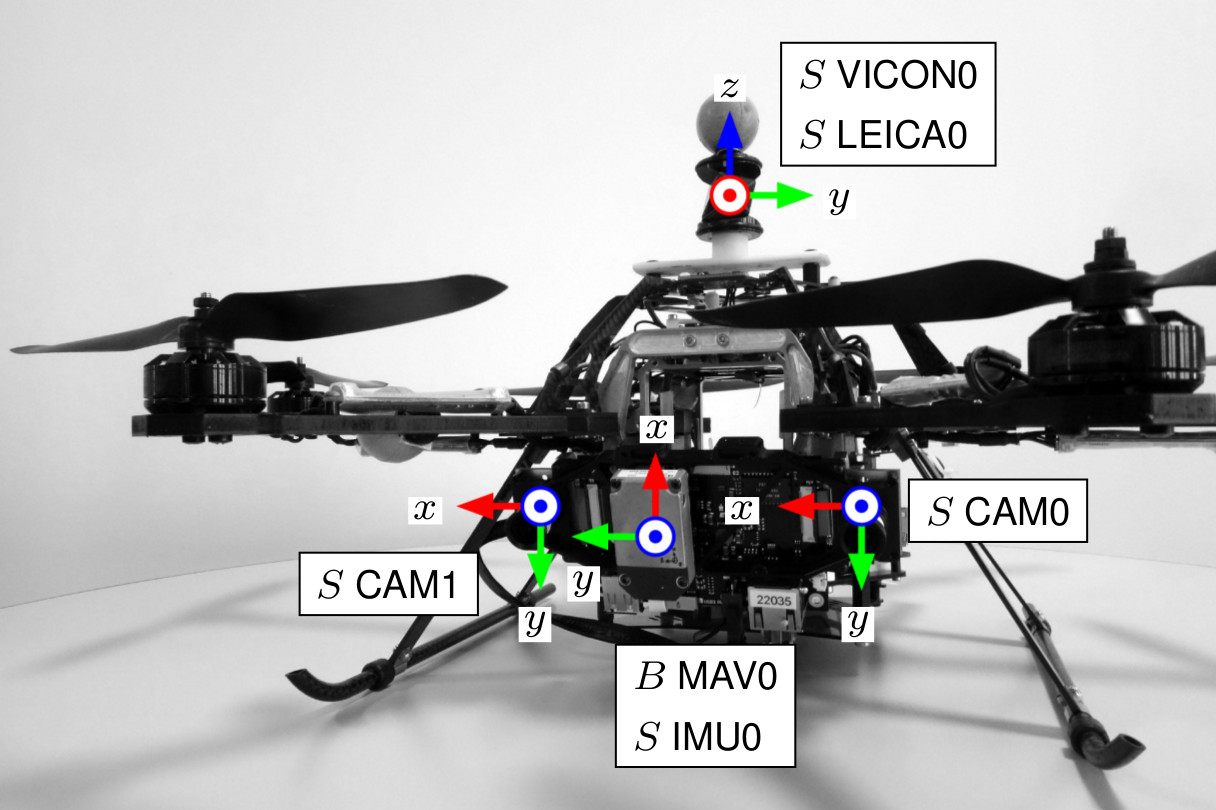
\includegraphics [width=0.35\textwidth]{figures/chapter5/fig5_1_1}}
	\hspace{0.5cm}
	\subfigure[]{
		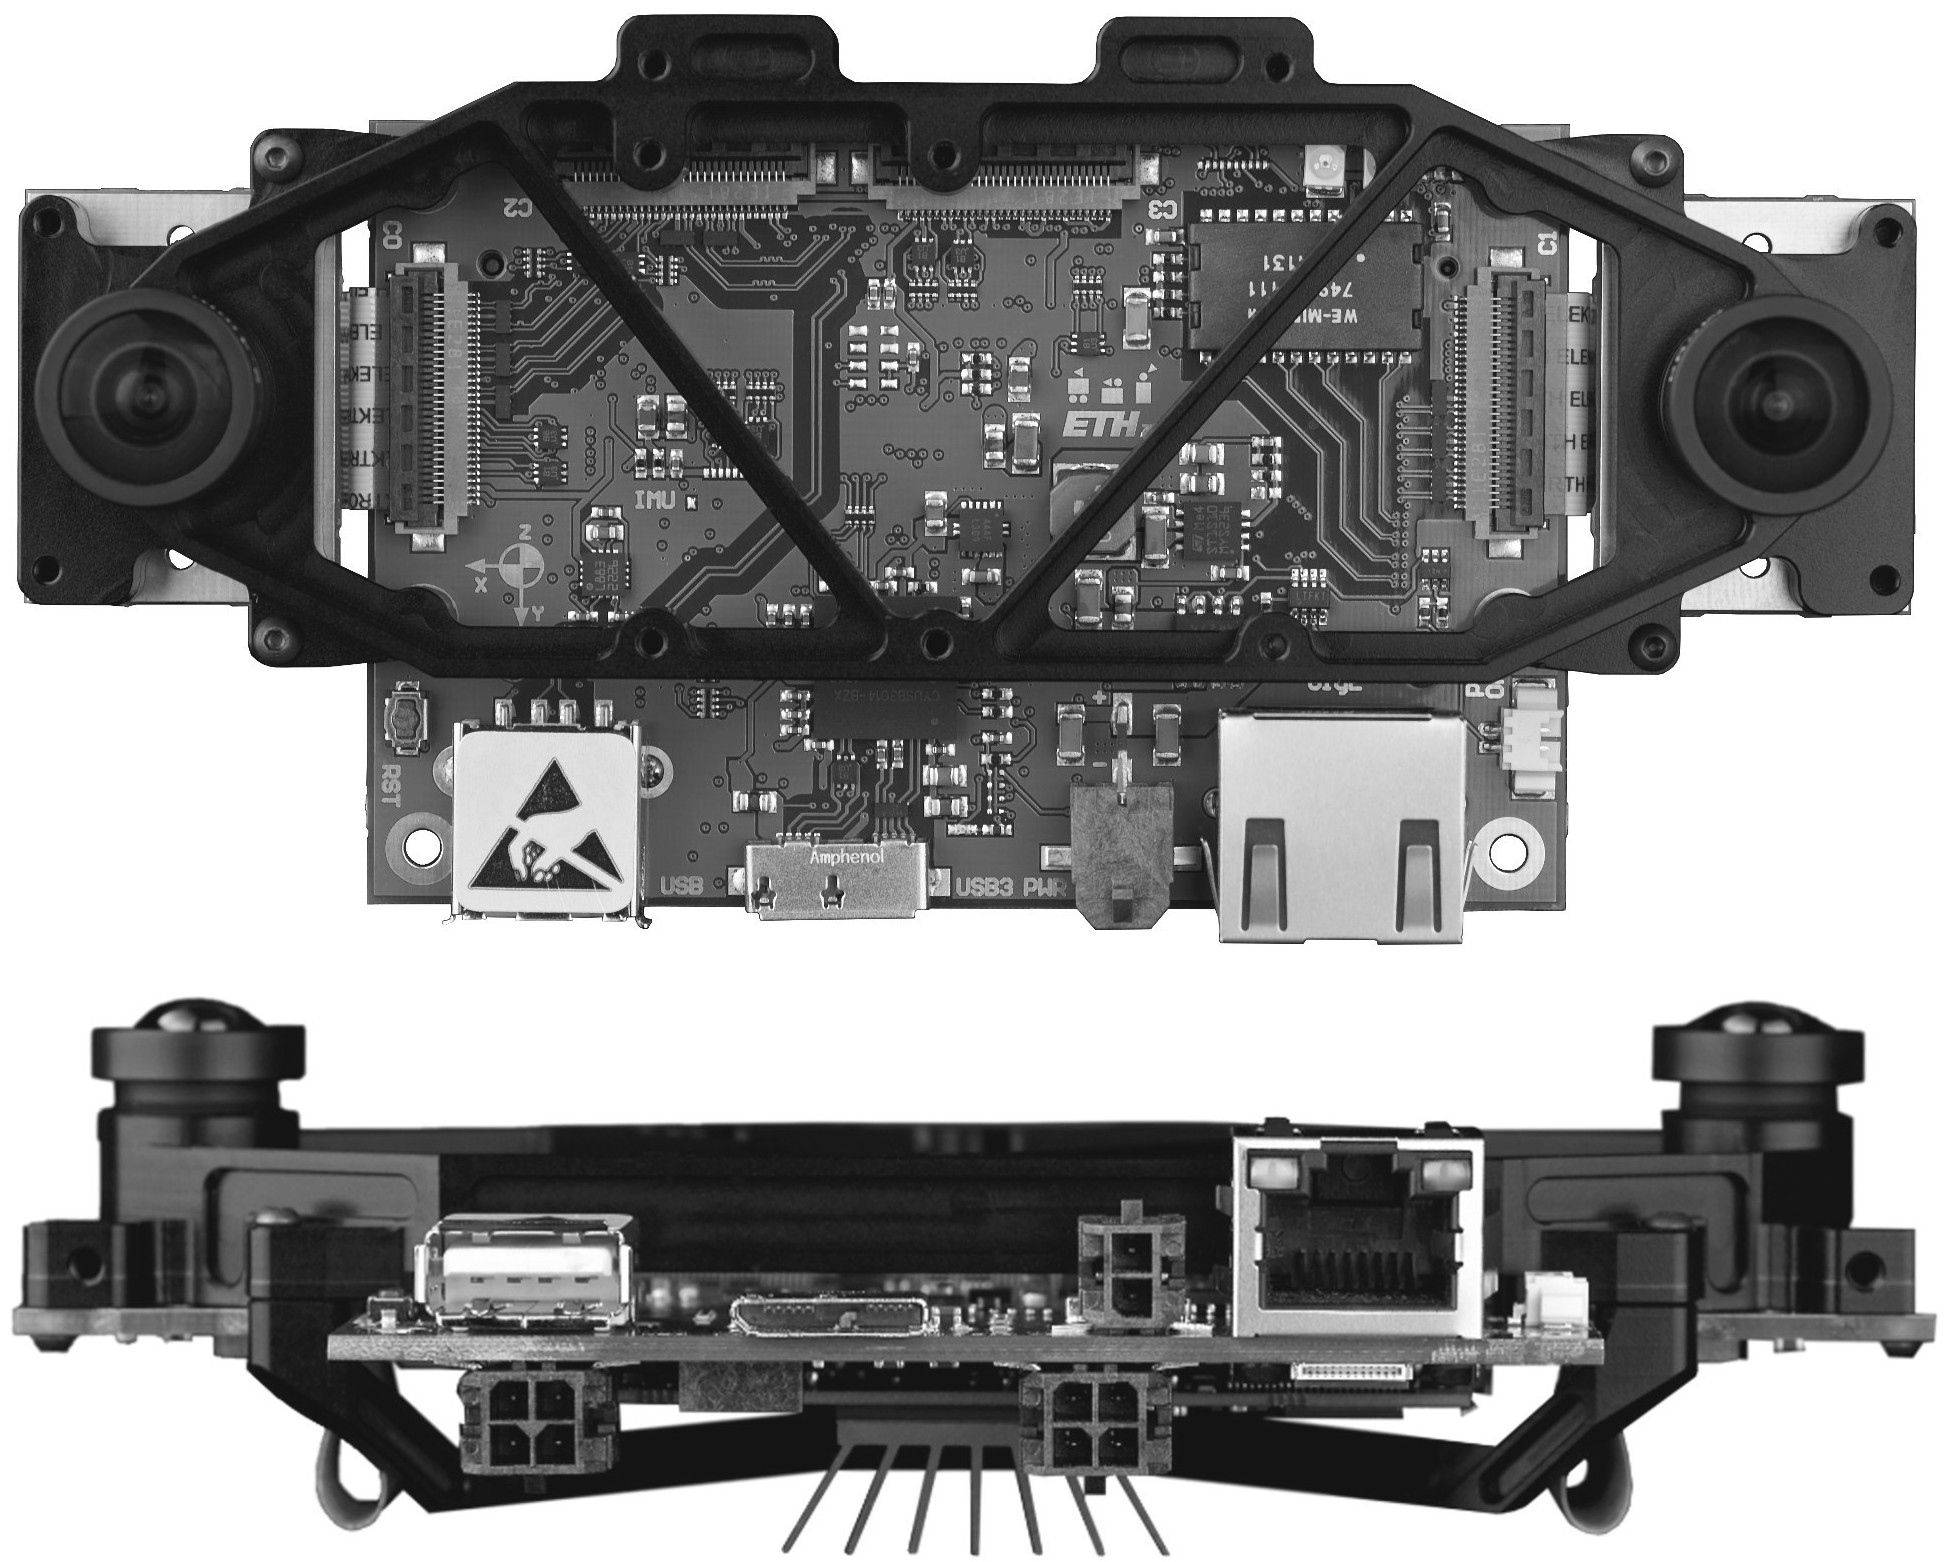
\includegraphics [width=0.35\textwidth]{figures/chapter5/fig5_1_2}}
	\caption{EuRoc硬件平台} \label{fig5_1}
\end{figure}

\begin{figure}[h]\setlength{\belowcaptionskip}{-12pt}
	\centering
	\subfigure[]{
	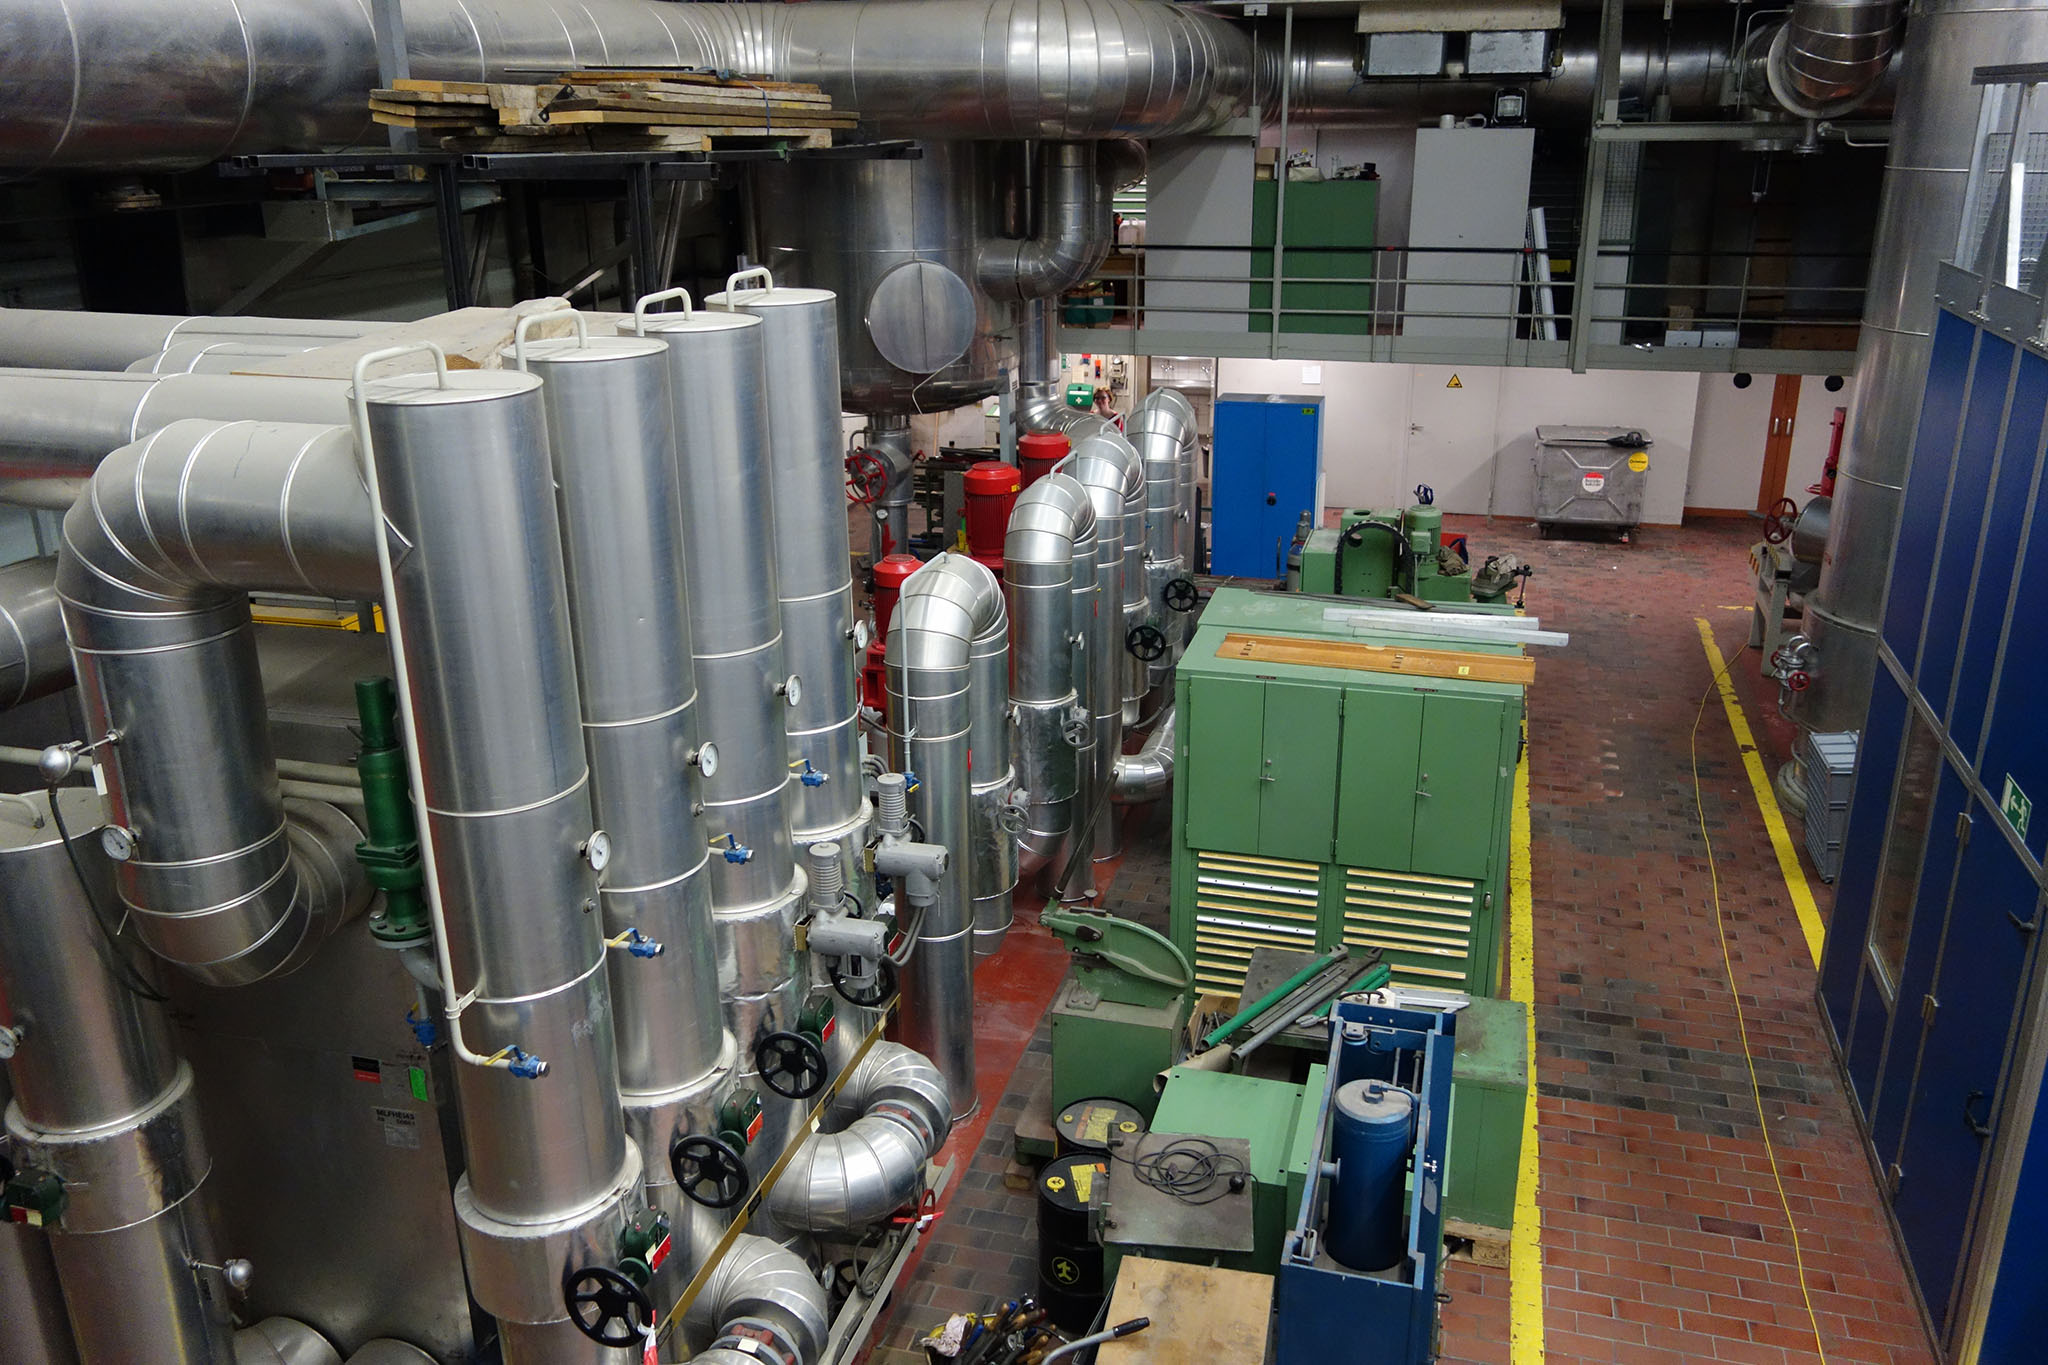
\includegraphics [width=0.42\textwidth]{figures/chapter5/fig5_2_1}}
	\hspace{0.5cm}
	\subfigure[]{
	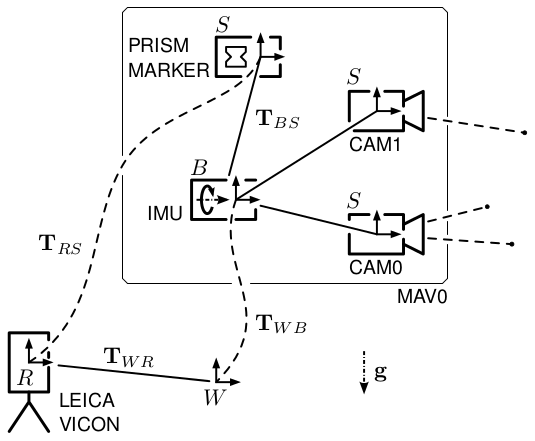
\includegraphics [width=0.35\textwidth]{figures/chapter5/fig5_2_2}}
	\caption{(a)机器大厅环境;(b)传感器和地面真值测量仪器之间的位置示意图} \label{fig5_2}
\end{figure}
\subsection{EuRoc实验一}
首先使用MH\_01\_easy进行实验。图\ref{fig5_3}是三维定位轨迹图对比图,图\ref{fig5_4}是三轴位置(x, y, z)对比图,图\ref{fig5_5}是三轴姿态(roll, pitch, yaw)对比图。其中VI\_SLAM是本系统输出轨迹,GroundTruth是数据集中的真值轨迹。通过图\ref{fig5_3},图\ref{fig5_4}和图\ref{fig5_5},可以定性分析系统的定位误差。
\begin{figure}
	\centering
	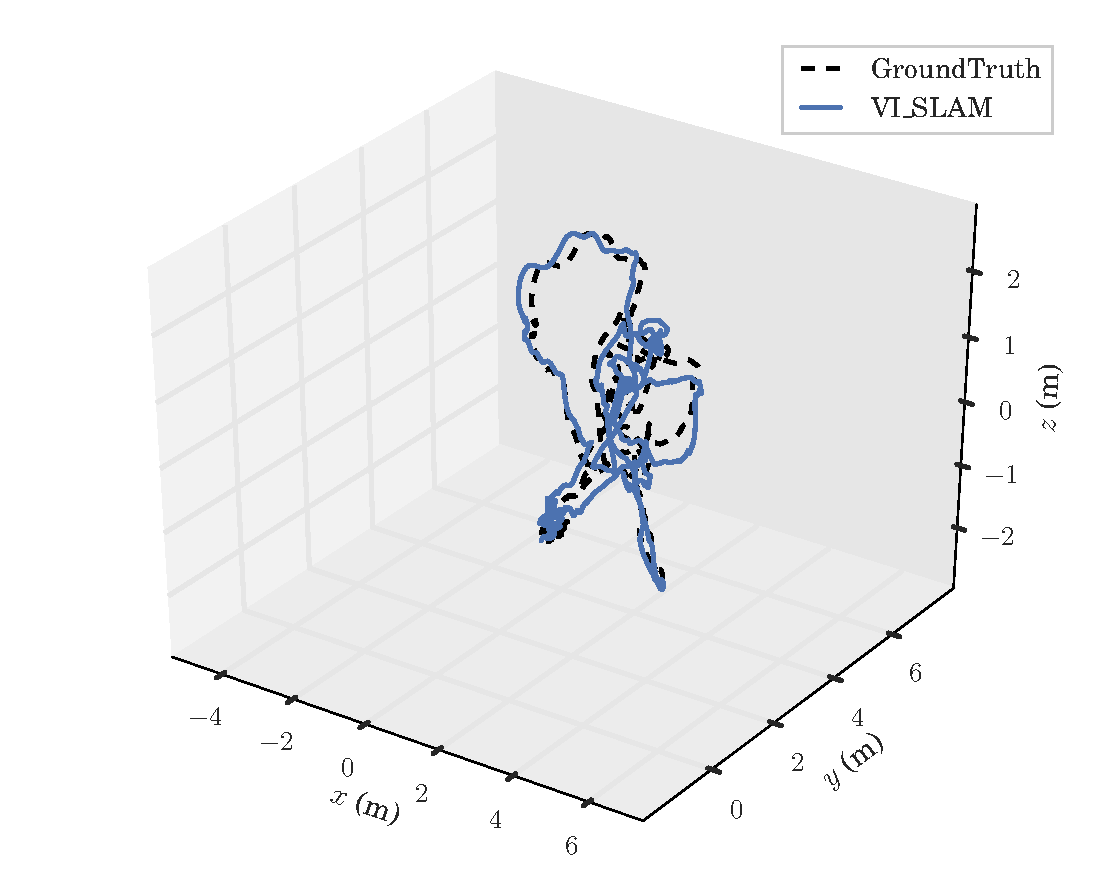
\includegraphics[width=0.7\textwidth]{figures/chapter5/traject_mh01}
	\caption{EuRoc实验一的三维定位轨迹图}\label{fig5_3}
\end{figure}
\begin{figure}
	\centering
	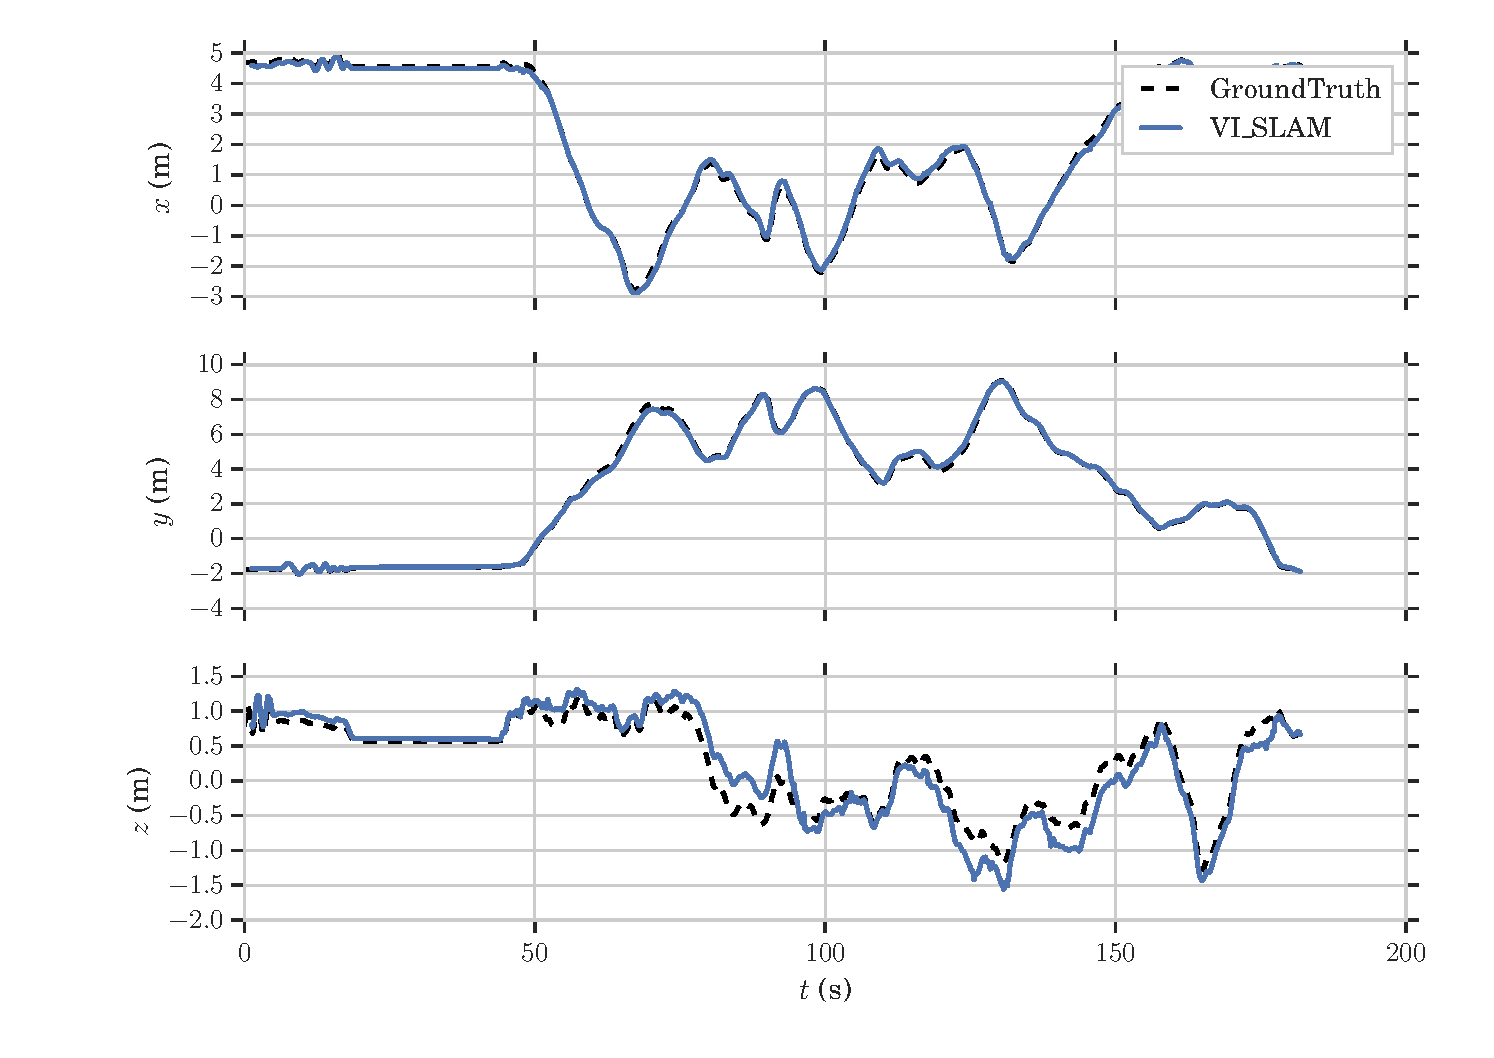
\includegraphics[width=1.0\textwidth]{figures/chapter5/xyz_mh01}
	\caption{EuRoc实验一的三轴位置(x, y, z)对比图}\label{fig5_4}
\end{figure}
\begin{figure}[!h]
	\centering
	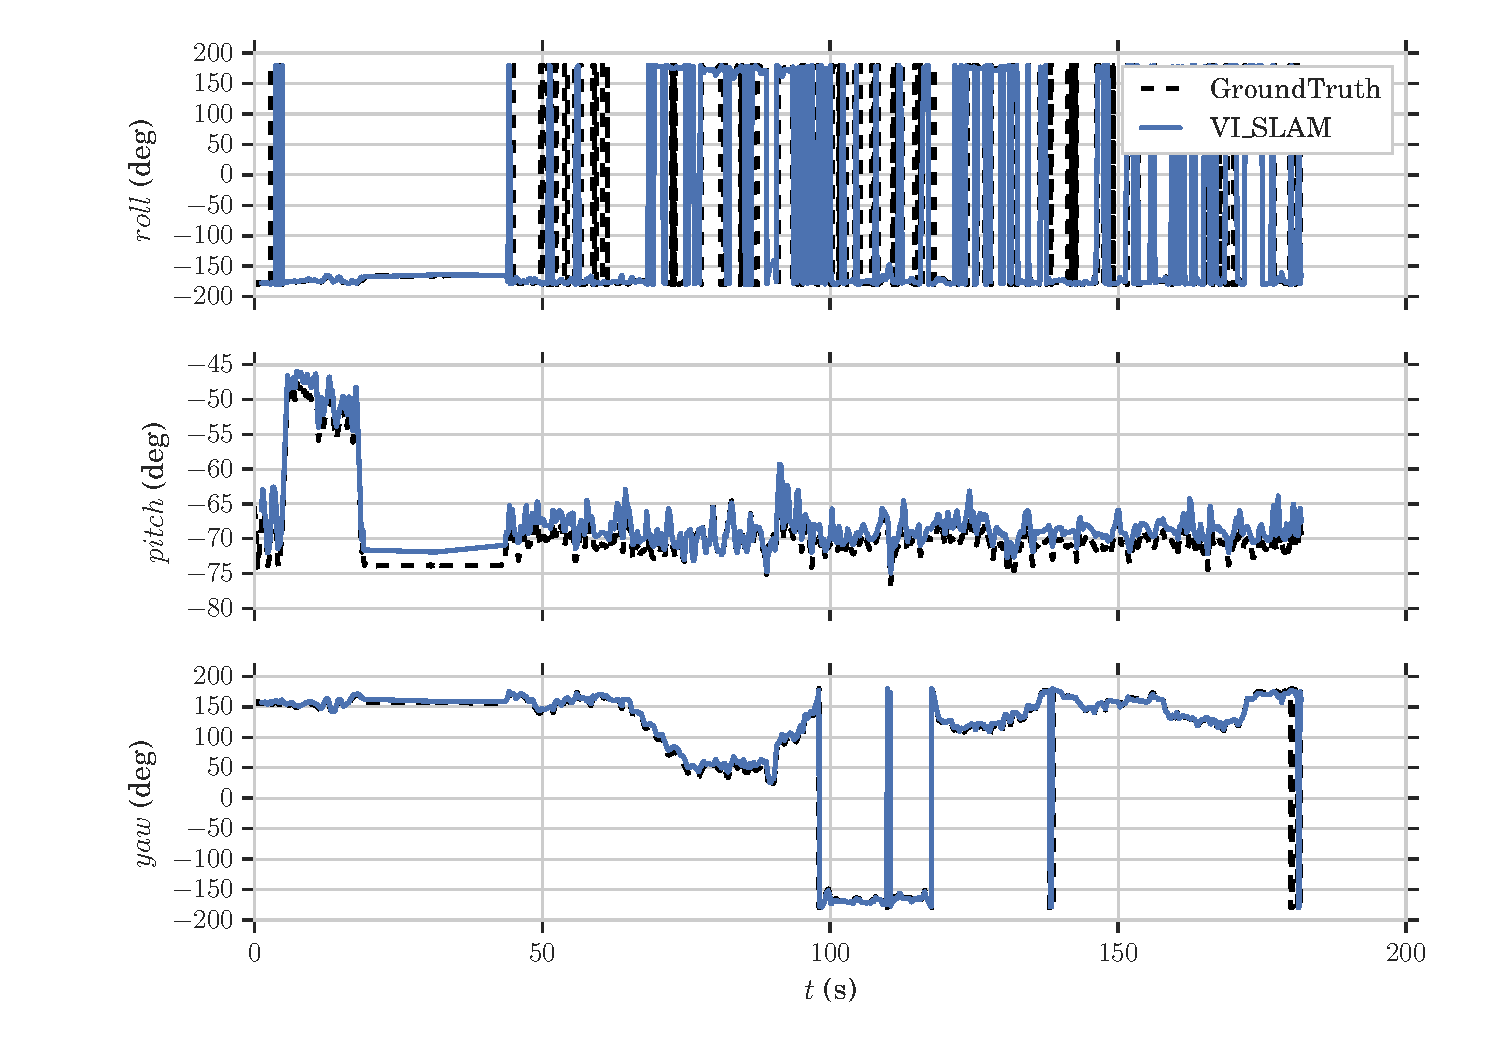
\includegraphics[width=1.0\textwidth]{figures/chapter5/rpy_mh01}
	\caption{EuRoc实验一的三轴姿态(roll, pitch, yaw)对比图}\label{fig5_5}
\end{figure}

然后定量分析EuRoc实验一中系统的定位误差。图\ref{fig5_6}是三维定位绝对误差图。计算出系统定位的绝对误差(APE),均方根误差(RMSE),标准差(STD),平均误差(MEAN)和中值误差(MEDIAN),将计算结果展示在表\ref{tab:5.1}中。为了更加直观,将这些误差以曲线图的形式展示出来,如图\ref{fig5_7}所示。
\begin{figure}[!h]
	\centering
	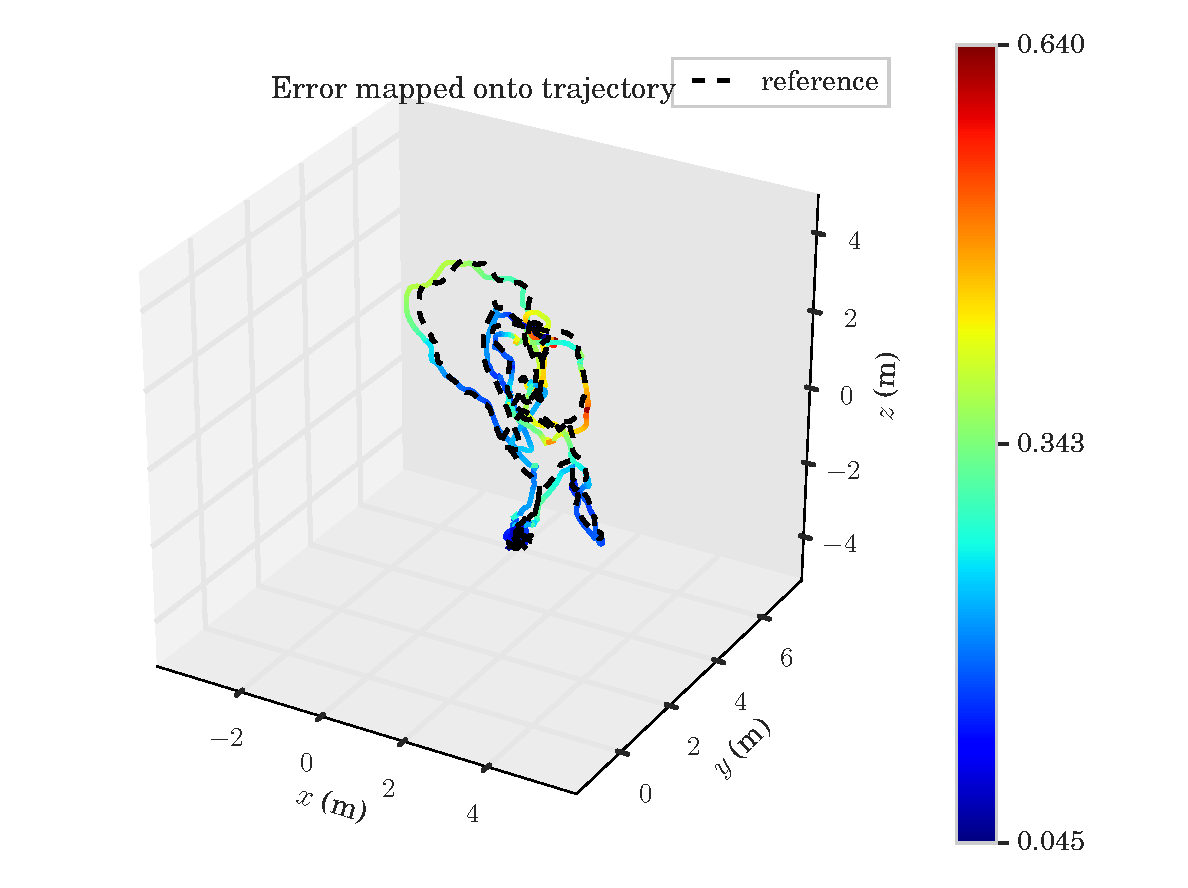
\includegraphics[width=0.7\textwidth]{figures/chapter5/ape_map_mh01}
	\caption{EuRoc实验一的三维定位绝对误差图}\label{fig5_6}
\end{figure}
\begin{figure}
	\centering
	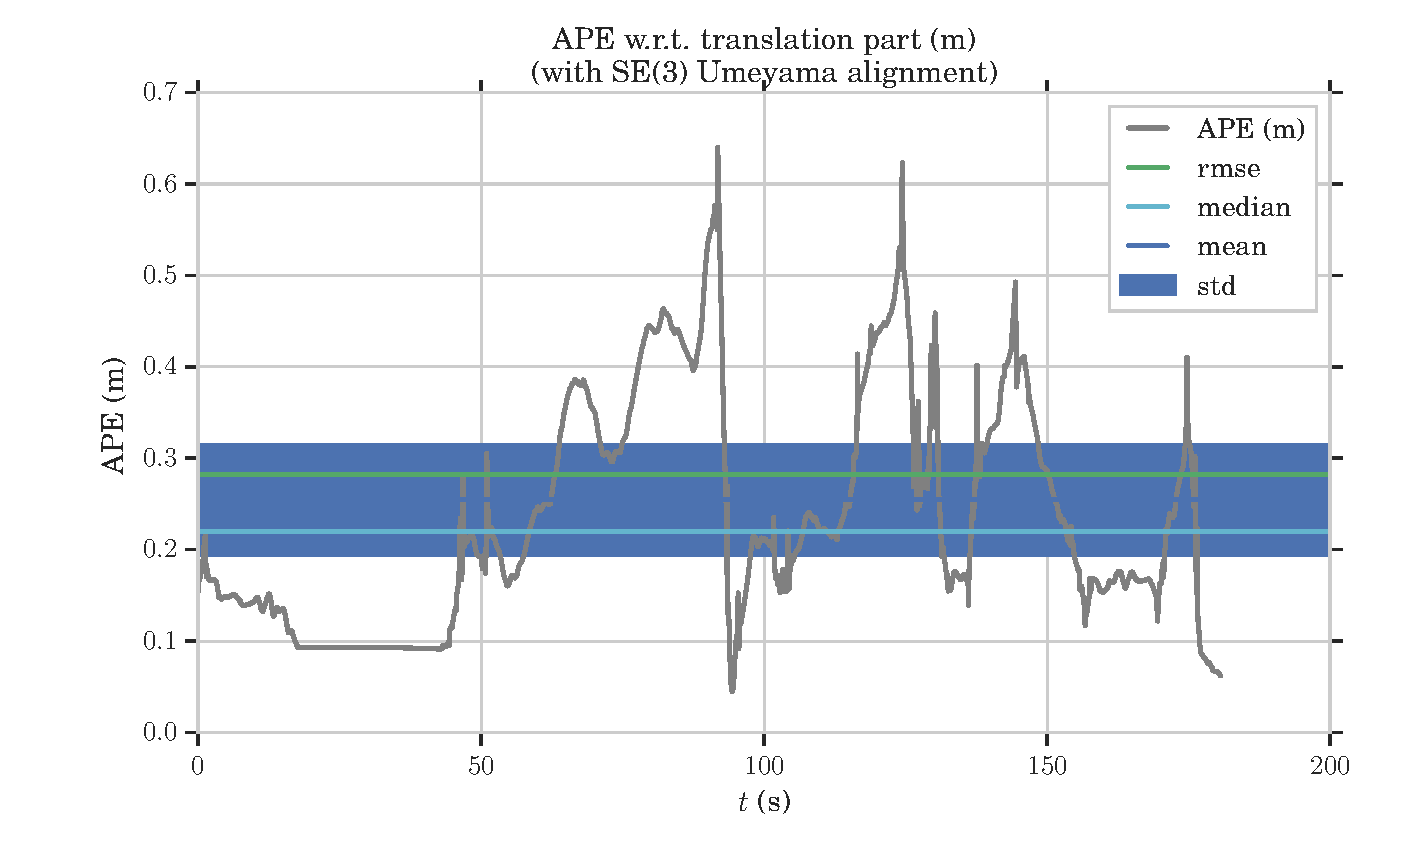
\includegraphics[width=1.0\textwidth]{figures/chapter5/ape_err_mh01}
	\caption{EuRoc实验一的系统定位误差指标图}\label{fig5_7}
\end{figure}
\begin{table}[!h]
	\zihao{5}
	\centering
	\caption{EuRoc实验一的系统定位误差指标} \label{tab:5.1}
	\begin{tabular*}{0.9\textwidth}{@{\extracolsep{\fill}}cccccc}
		\toprule
		APE\_MAX(m)&APE\_MIN(m) &RMSE	&STD	&MEAN(m)	&MEDIAN(m) \\
		\midrule
		0.6403	&0.0447	&0.2820	&0.1212	&0.2546	&0.2199\\
		\bottomrule
	\end{tabular*}
\end{table}

对比其他开源VIO方案在MH\_01\_easy上的误差的RMSE\upcite{delmerico2018benchmark},MSCKF为0.43,OKVIS为0.16,ROVIO为0.21,可见本系统在MH\_01\_easy上的定位精度介于MSCKF和ROVIO之间。
\subsection{EuRoc实验二}
使用MH\_05\_difficult数据集进行实验。图\ref{fig5_8}是三维定位轨迹图对比图,图\ref{fig5_9}是三轴位置(x, y, z)对比图,图\ref{fig5_10}是三轴姿态(roll, pitch, yaw)对比图。其中VI\_SLAM是本系统输出轨迹,GroundTruth是数据集中的真值轨迹。通过图\ref{fig5_8},图\ref{fig5_9}和图\ref{fig5_10},可以定性分析系统的定位误差。
\begin{figure}
	\centering
	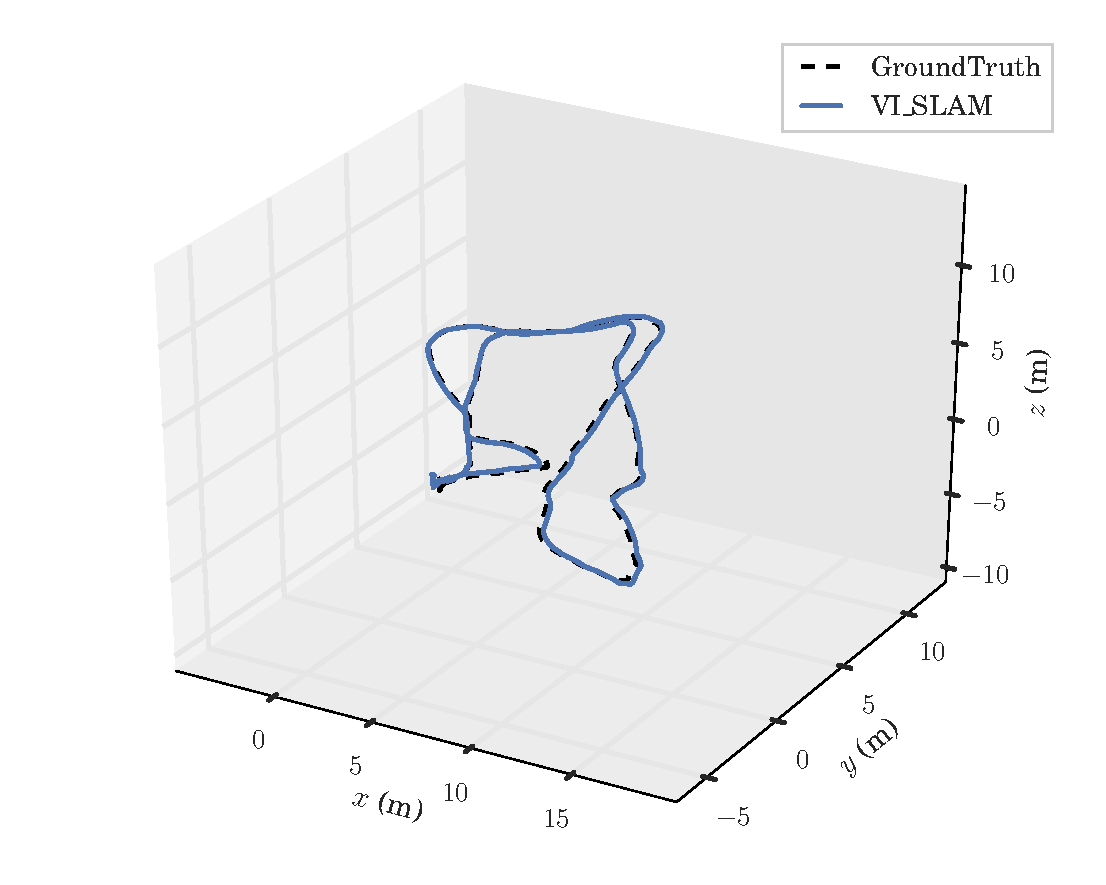
\includegraphics[width=0.7\textwidth]{figures/chapter5/traject_mh05}
	\caption{EuRoc实验二的三维定位轨迹图}\label{fig5_8}
\end{figure}
\begin{figure}
	\centering
	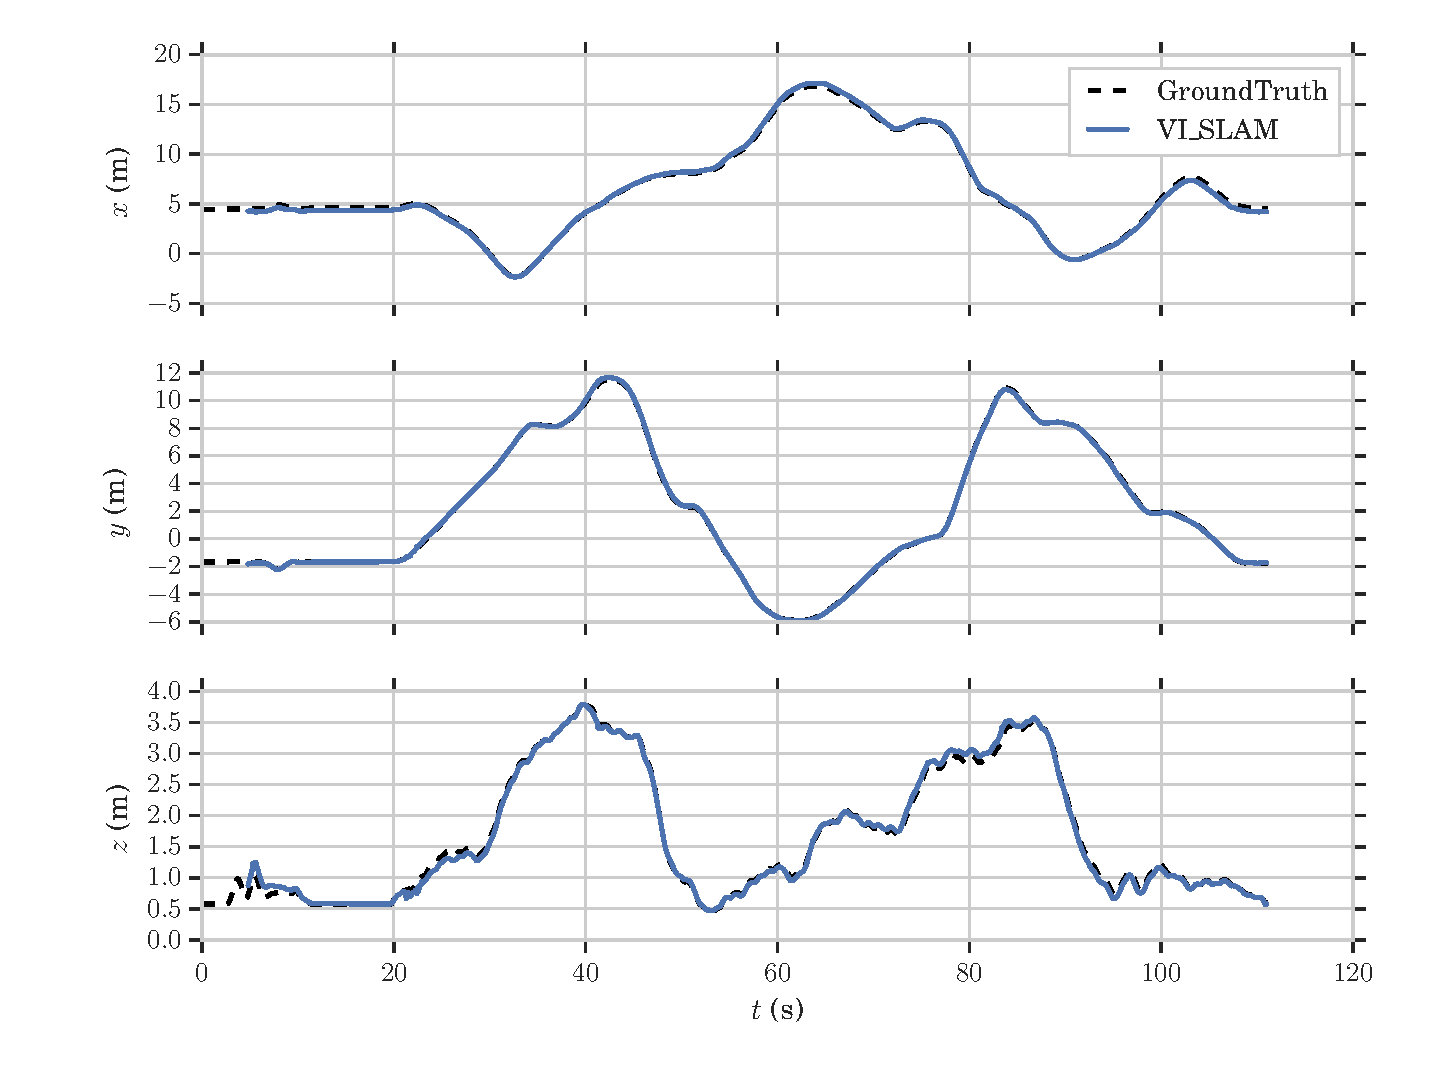
\includegraphics[width=1.0\textwidth]{figures/chapter5/xyz_mh05}
	\caption{EuRoc实验二的三轴位置(x, y, z)对比图}\label{fig5_9}
\end{figure}
\begin{figure}[!h]
	\centering
	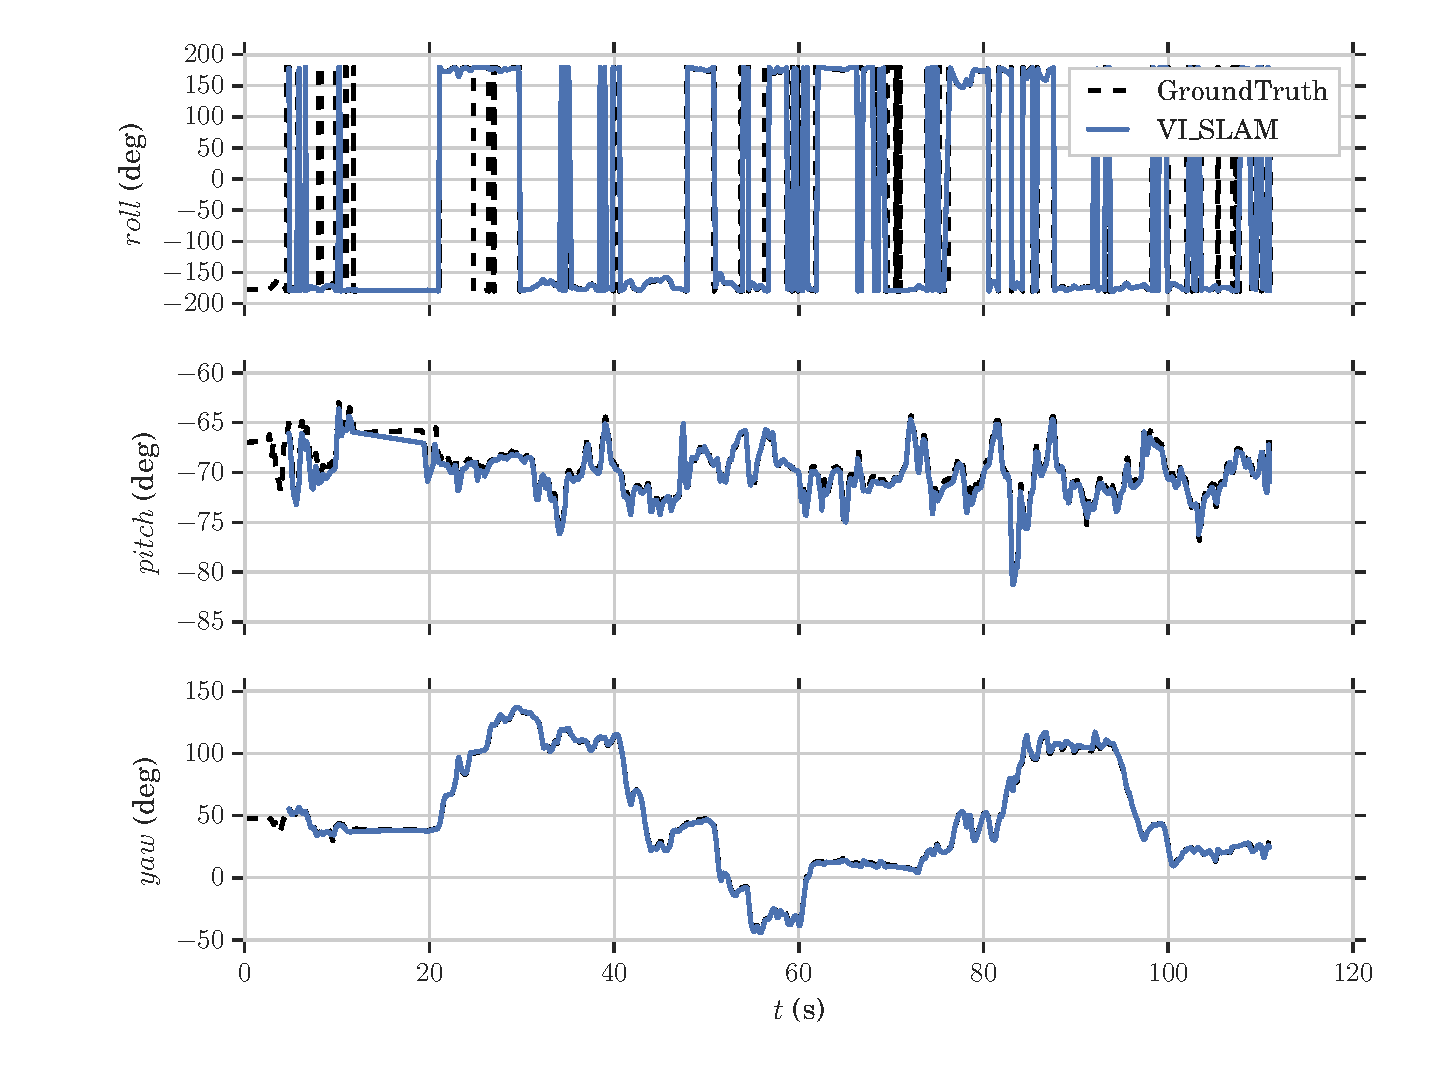
\includegraphics[width=1.0\textwidth]{figures/chapter5/rpy_mh05}
	\caption{EuRoc实验二的三轴姿态(roll, pitch, yaw)对比图}\label{fig5_10}
\end{figure}

然后定量分析EuRoc实验二中系统的定位误差。图\ref{fig5_11}是三维定位绝对误差图。同样,计算出APE,RMSE,STD,MEAN和MEDIAN,将计算结果展示在表\ref{tab:5.2}中。为了更加直观,将这些误差以曲线图的形式展示出来,如图\ref{fig5_12}所示。\newpage
\begin{figure}[!h]\setlength{\belowcaptionskip}{-12pt}
	\centering
	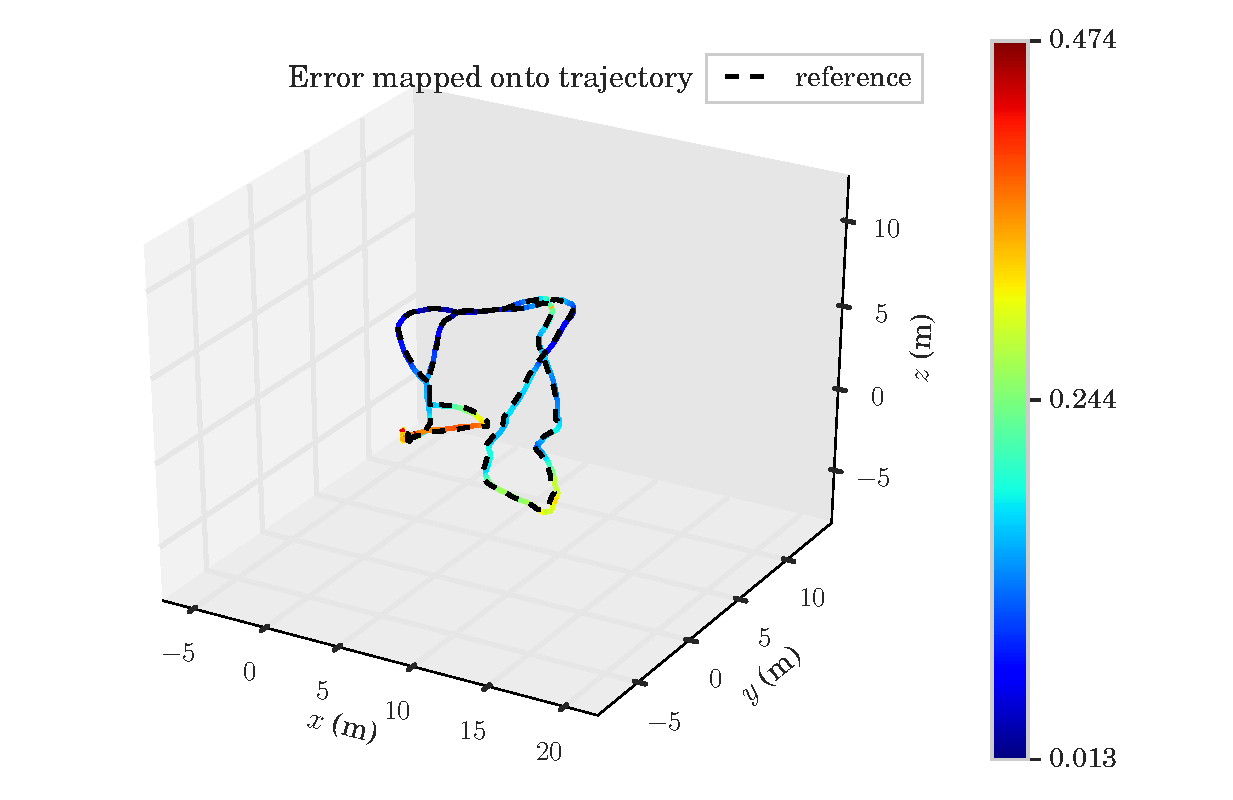
\includegraphics[width=0.75\textwidth]{figures/chapter5/ape_map_mh05}
	\caption{EuRoc实验二的三维定位绝对误差图}\label{fig5_11}
\end{figure}
\begin{figure}[!h]\setlength{\belowcaptionskip}{-12pt}
	\centering
	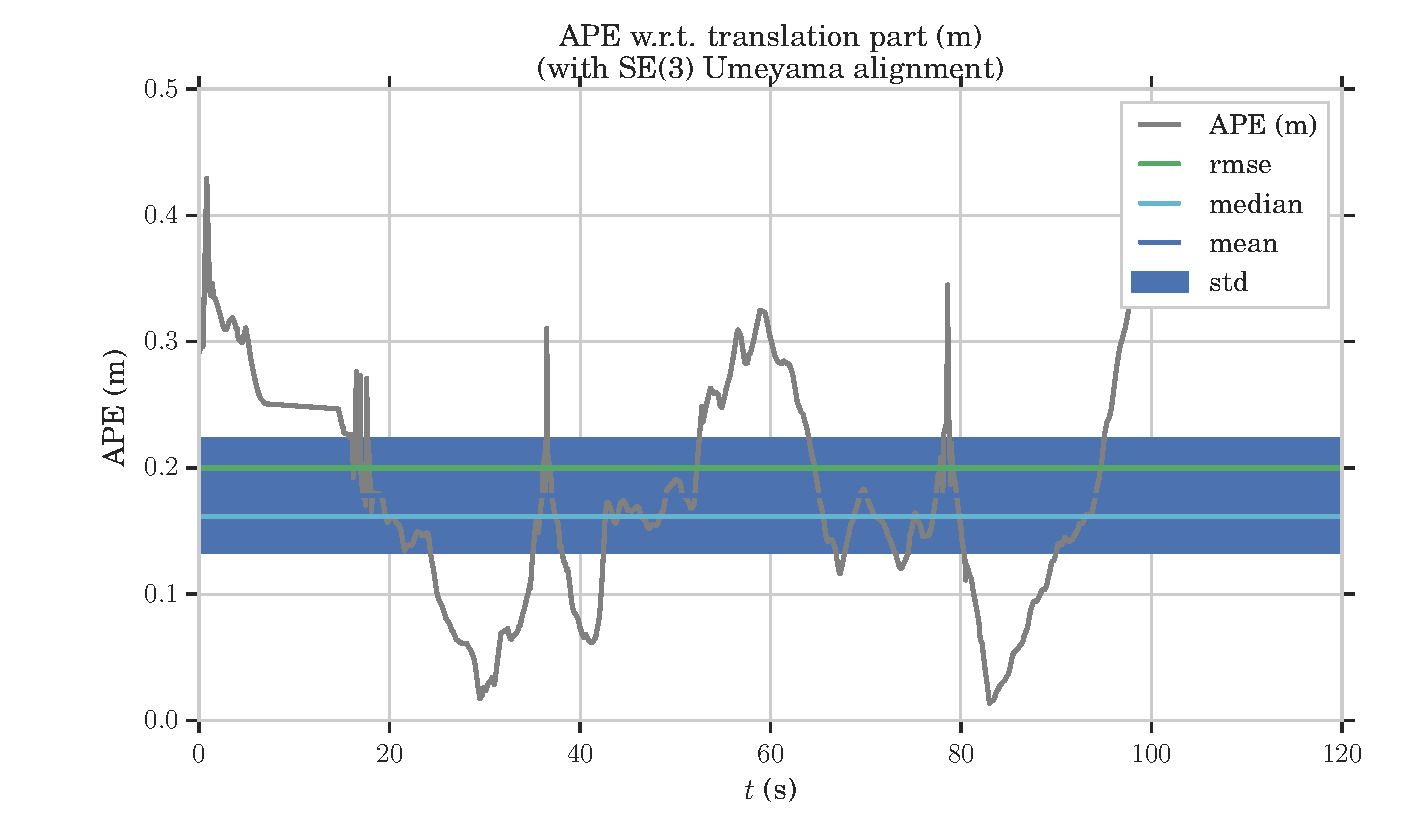
\includegraphics[width=1.0\textwidth]{figures/chapter5/ape_err_mh05}
	\caption{EuRoc实验二的系统定位误差指标图}\label{fig5_12}
\end{figure}
\begin{table}[!h]\setlength{\abovecaptionskip}{6pt}
	\zihao{5}
	\centering
	\caption{EuRoc实验二的系统定位误差指标} \label{tab:5.2}
	\begin{tabular*}{0.9\textwidth}{@{\extracolsep{\fill}}cccccc}
		\toprule
		APE\_MAX(m)&APE\_MIN(m) &RMSE	&STD	&MEAN(m)	&MEDIAN(m) \\
		\midrule
		0.4739	&0.0134	&0.1999	&0.0901	&0.1784	&0.1616\\
		\bottomrule
	\end{tabular*}
\end{table}

对比其他开源VIO方案在MH\_05\_difficult上的误差的RMSE\upcite{delmerico2018benchmark},MSCKF为0.48,OKVIS为0.56,ROVIO为0.52,可见本系统在MH\_01\_difficult上的定位精度要远远高于其他开源方案。这也说明了本系统更加适应复杂环境,鲁棒性更高。
\section{本地实时实验}
\subsection{本地实验硬件及环境}
使用实验室的丰田SUV进行车载实验,如图\ref{fig5_13}(a)所示。图\ref{fig5_13}(b)是搭载在车顶上的多传感器硬件系统,其具体构成已经在2.3.1小节中介绍。
\begin{figure}[h]\setlength{\belowcaptionskip}{-12pt}
	\centering
	\subfigure[]{
	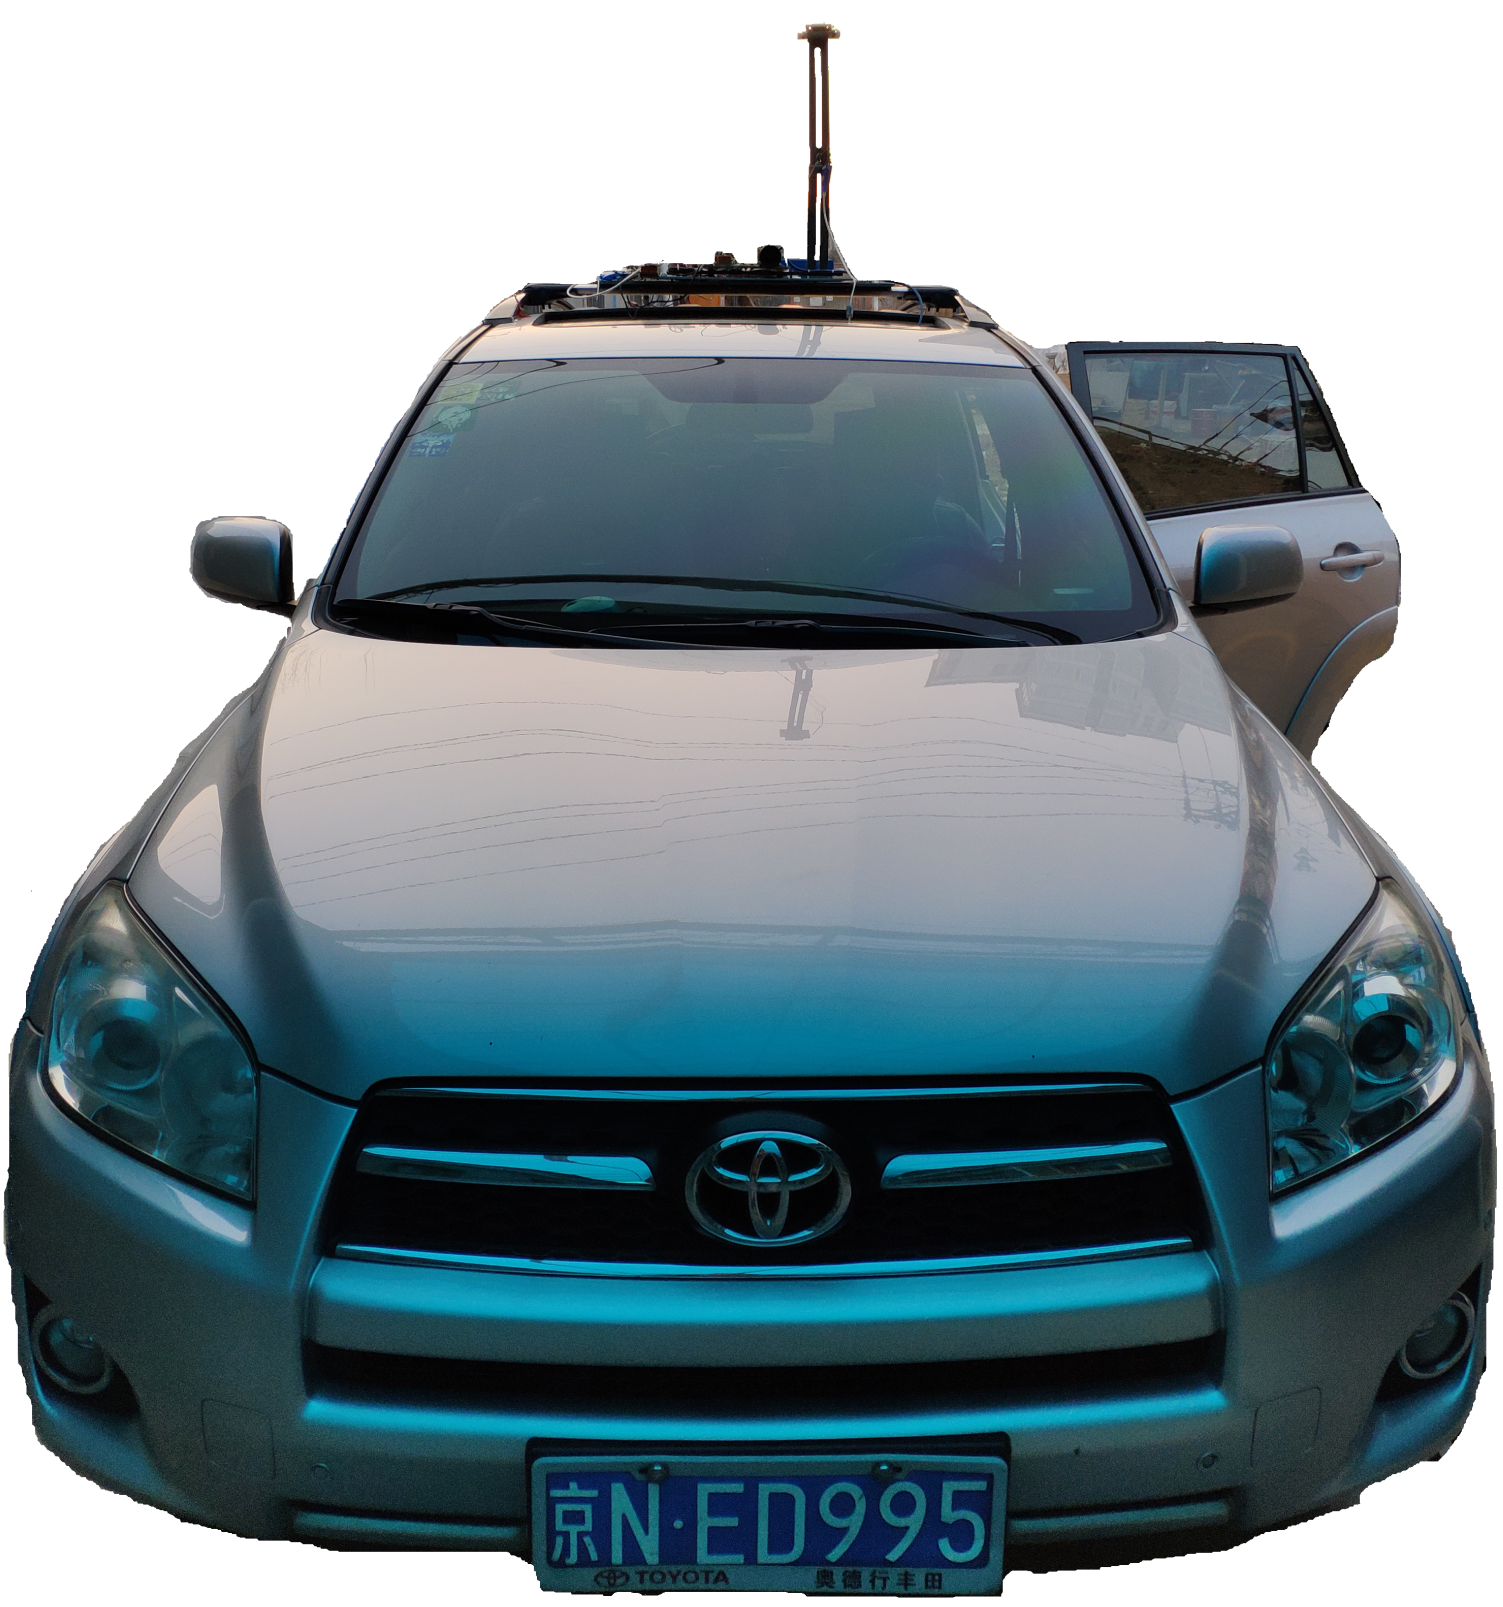
\includegraphics [width=0.3\textwidth]{figures/chapter5/fig5_13_1}}
	\hspace{0.5cm}
	\subfigure[]{
	\includegraphics [width=0.25\textwidth]{figures/chapter5/fig5_13_2}}
	\caption{本地实验设备} \label{fig5_13}
\end{figure}

本地车载实验的路线有两个,一个是环绕半个北京理工大学中关村校区,大约2.8km,如图\ref{fig5_14}黄色GPS轨迹线所示。另一个是环绕整个北京理工大学中关村校区一周,大约4.3km,如图\ref{fig5_14}红色GPS轨迹线所示。
\begin{figure}[h]\setlength{\belowcaptionskip}{-12pt}
	\centering
	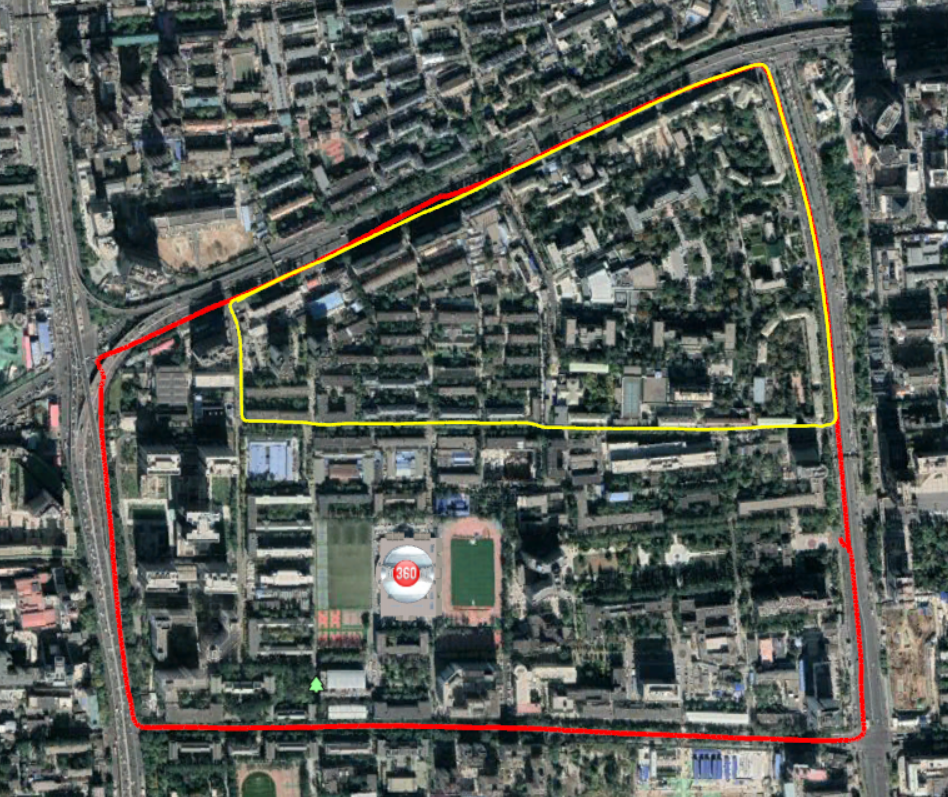
\includegraphics[width=0.45\textwidth]{figures/chapter5/fig5_14}
	\caption{车载实验路线}\label{fig5_14}
\end{figure}
由于是车载实验,所以本系统只关注2自由度(x,y)位置,忽略高度。本系统使用RTK采集经纬度信息,经过高斯投影后转化为WGS-84坐标,用这个坐标点轨迹作为真值数据。所以,本系统的真值数据也只有2自由度位置信息,没有姿态真值。
\subsection{本地实验一}
实验一的行车轨迹如图\ref{fig5_14}黄线所示。图\ref{fig5_15}是二维定位轨迹图对比图,图\ref{fig5_16}是二轴位置(x, y)对比图。其中VI\_SLAM是本系统输出轨迹,RTK是差分GPS轨迹。通过图\ref{fig5_15}和图\ref{fig5_16},可以定性分析系统的定位误差。
\begin{figure}[h]\setlength{\belowcaptionskip}{-12pt}
	\centering
	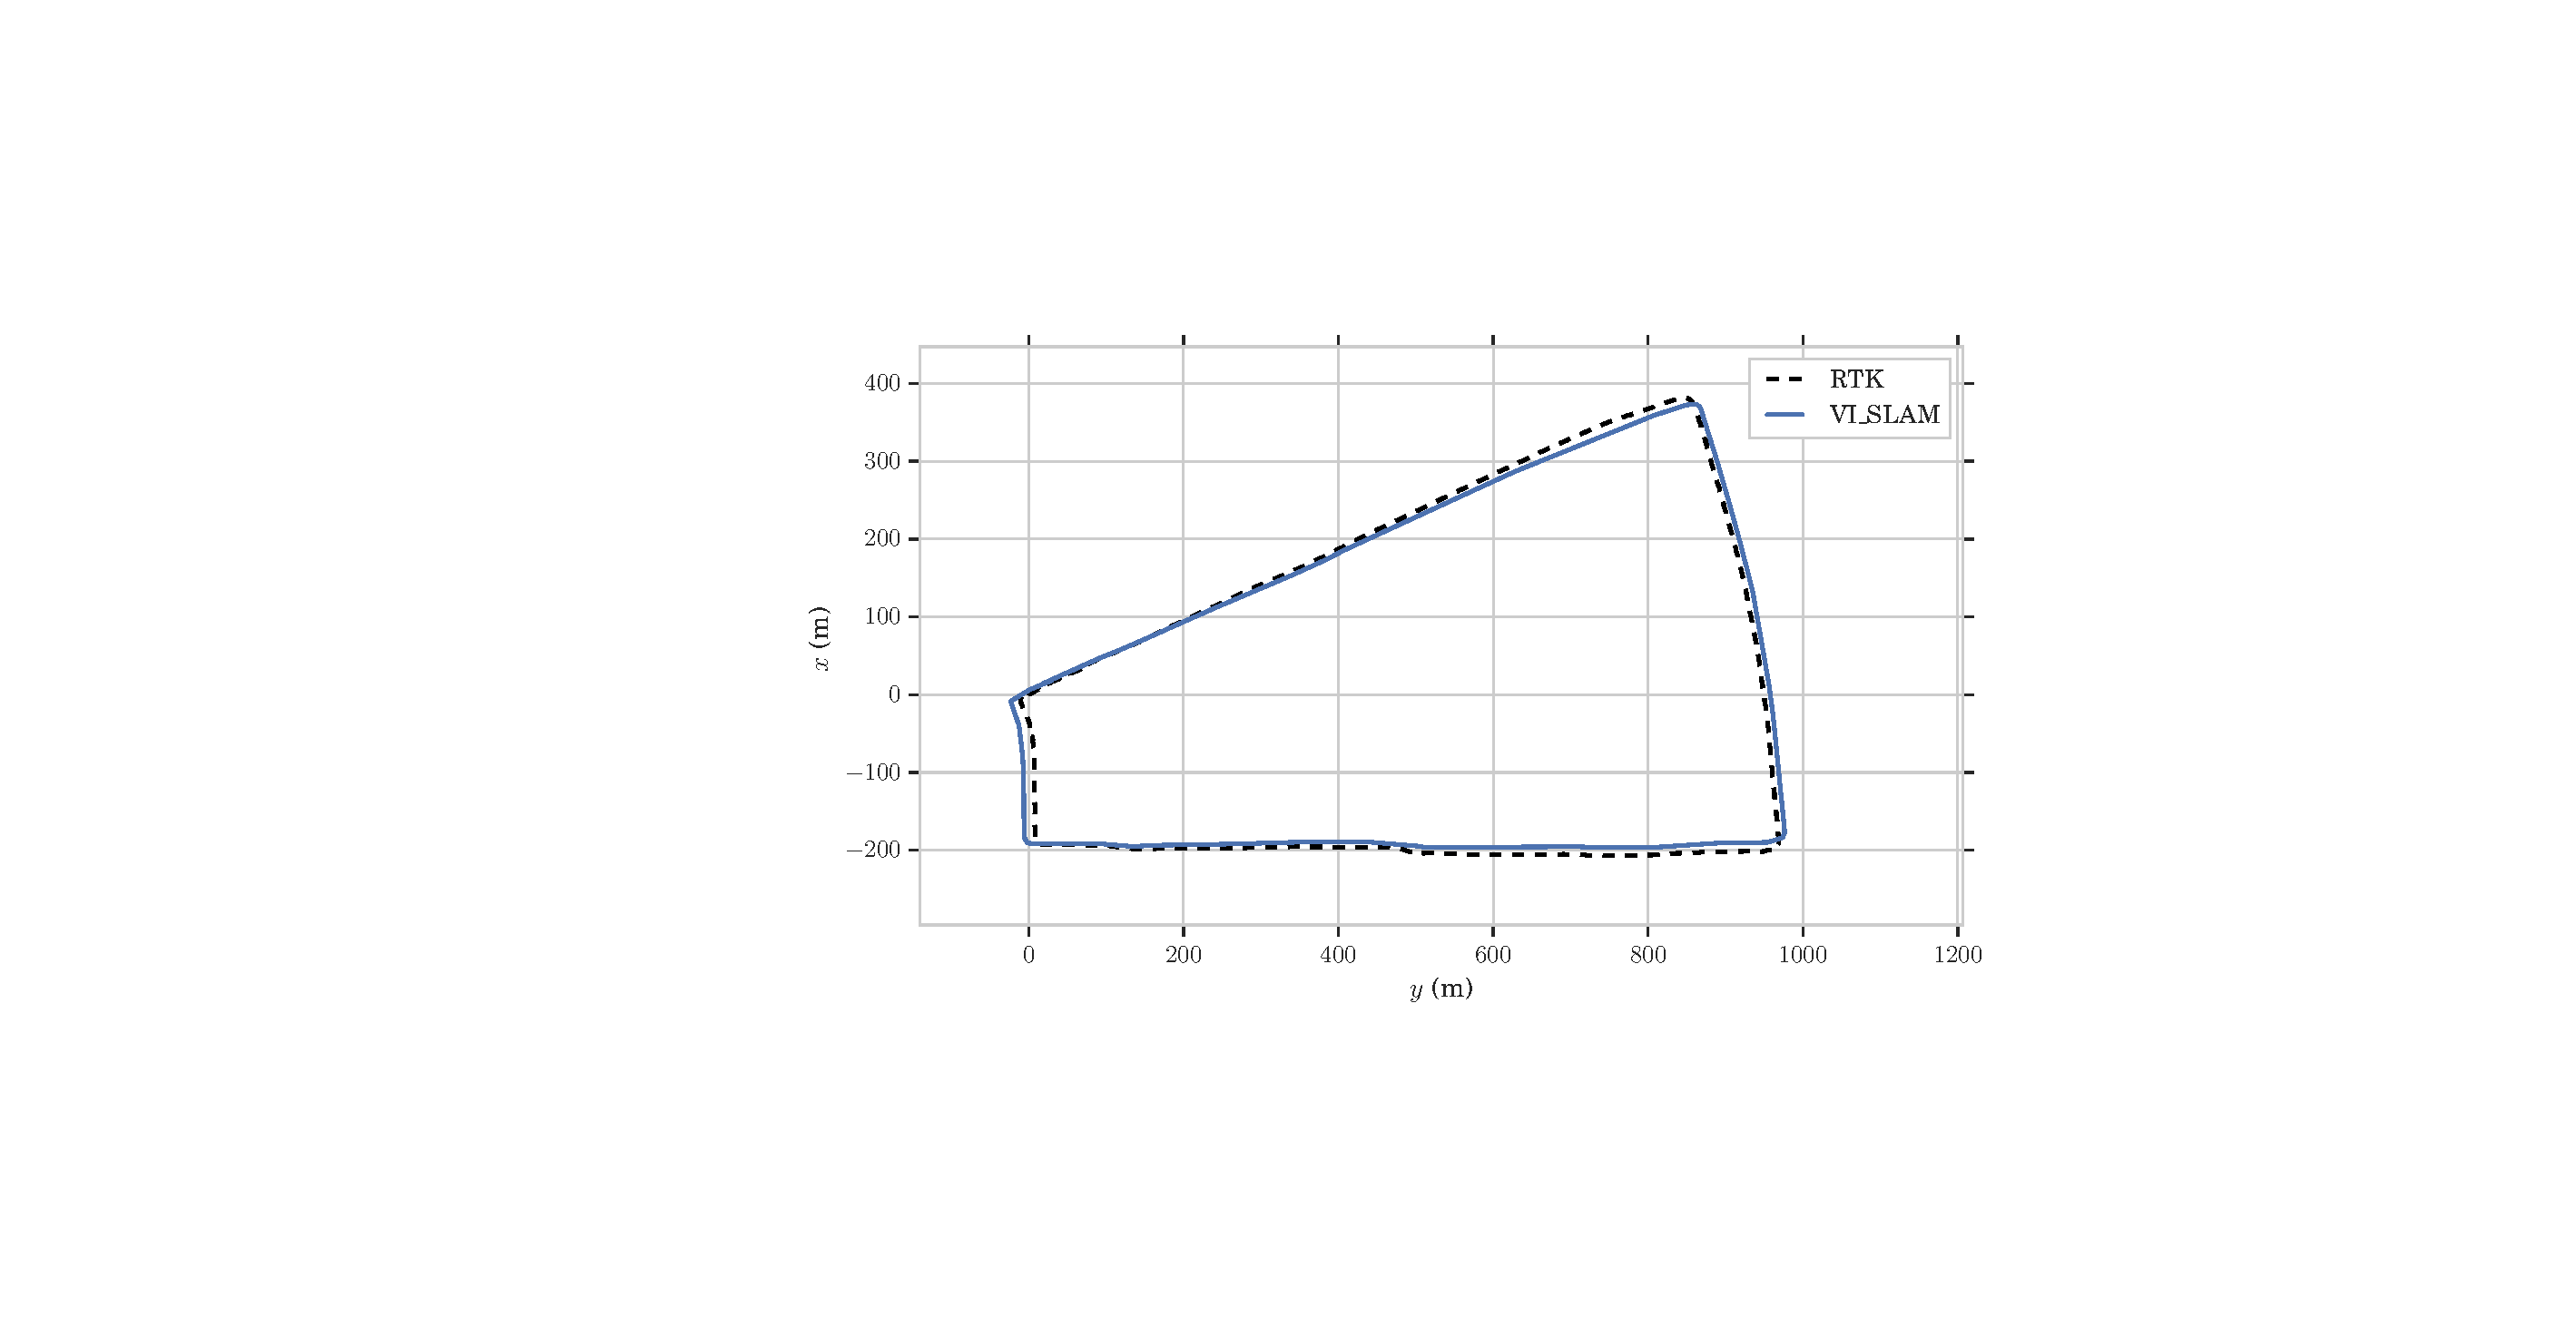
\includegraphics[width=0.90\textwidth]{figures/chapter5/traject_3km}
	\caption{本地实验一的二维定位轨迹图对比图}\label{fig5_15}
\end{figure}
\begin{figure}[h]\setlength{\belowcaptionskip}{-12pt}
	\centering
	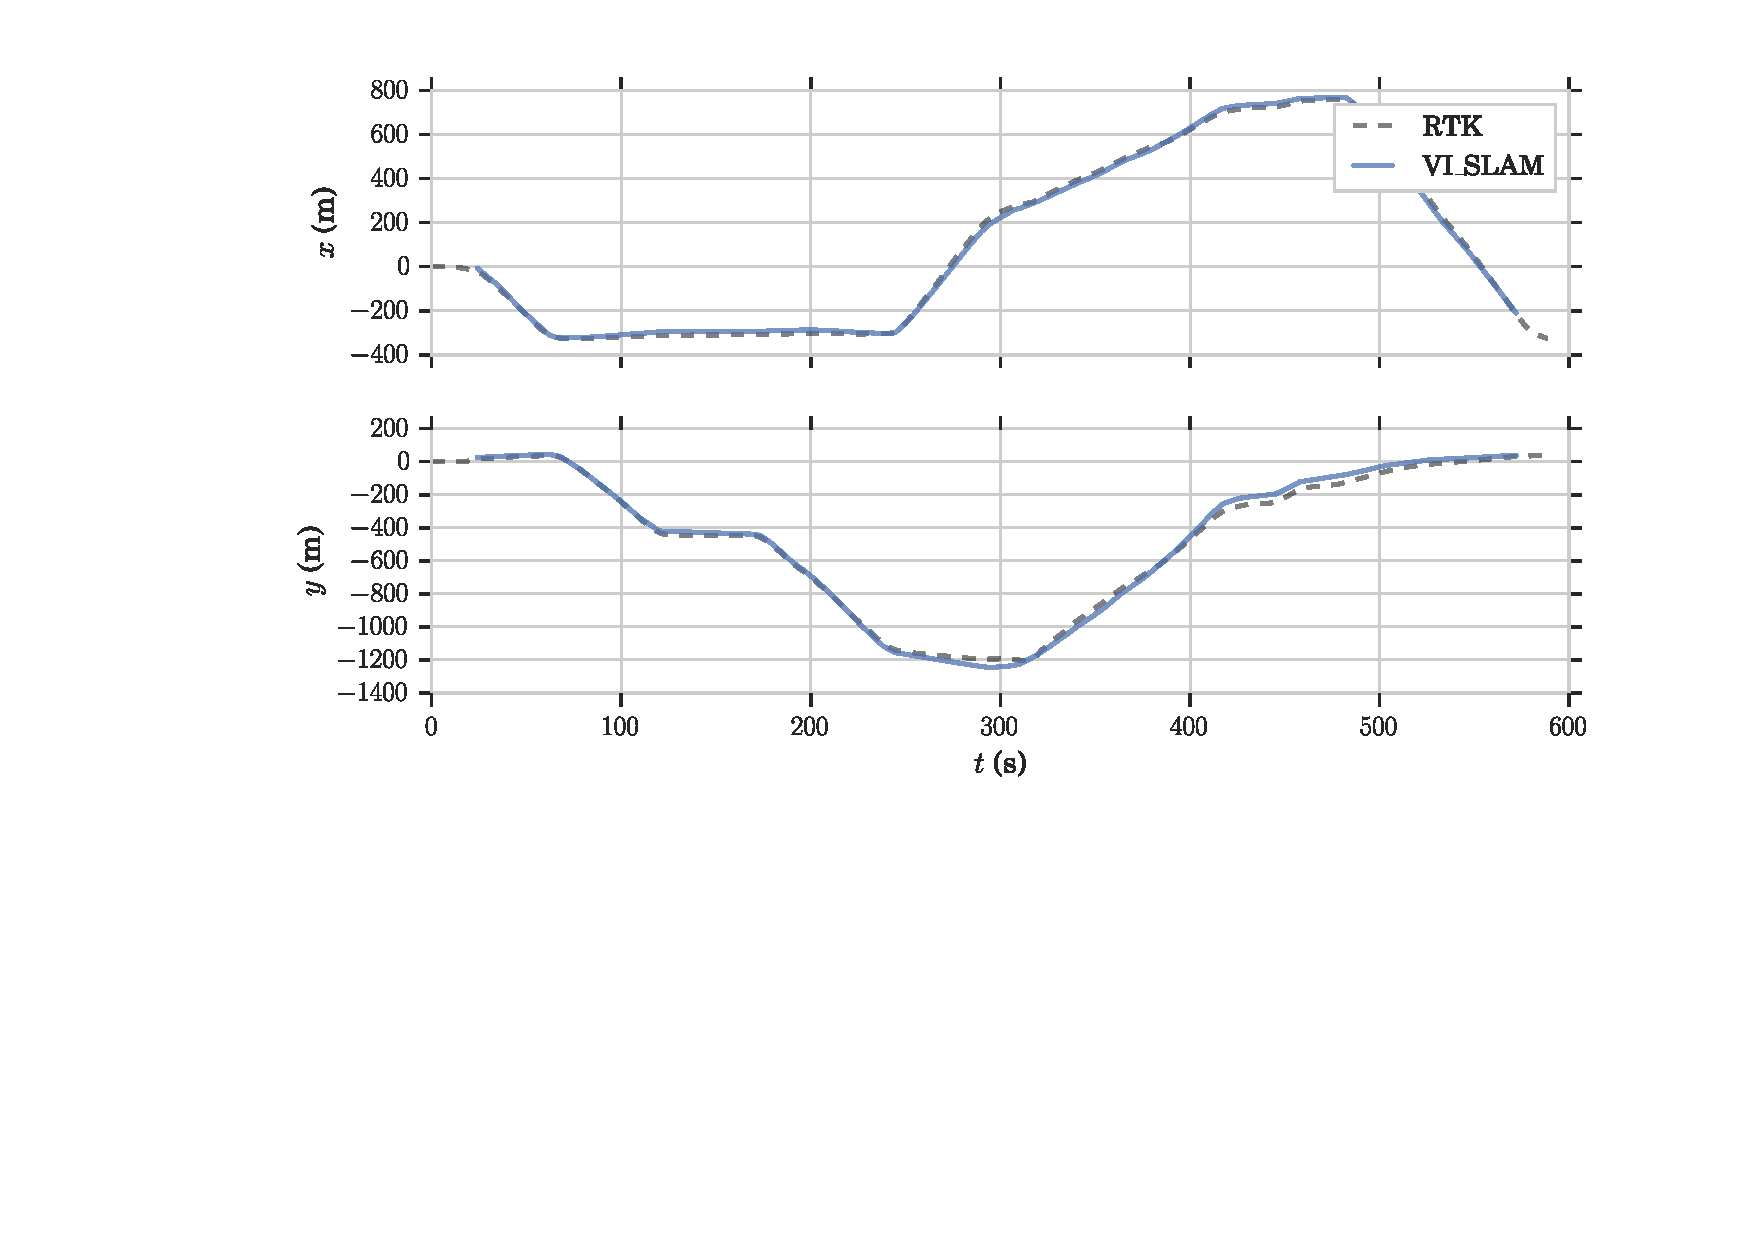
\includegraphics[width=1.0\textwidth]{figures/chapter5/xy_3km}
	\caption{本地实验一的二轴位置(x, y)对比图}\label{fig5_16}
\end{figure} 

然后定量分析本地实验一中系统的定位误差。图\ref{fig5_17}是二维定位绝对误差图。同样,计算出APE,RMSE,STD,MEAN和MEDIAN,将计算结果展示在表\ref{tab:5.3}中。为了更加直观,将这些误差以曲线图的形式展示出来,如图\ref{fig5_18}所示。\newpage
\begin{figure}[!h]\setlength{\belowcaptionskip}{-12pt}
	\centering
	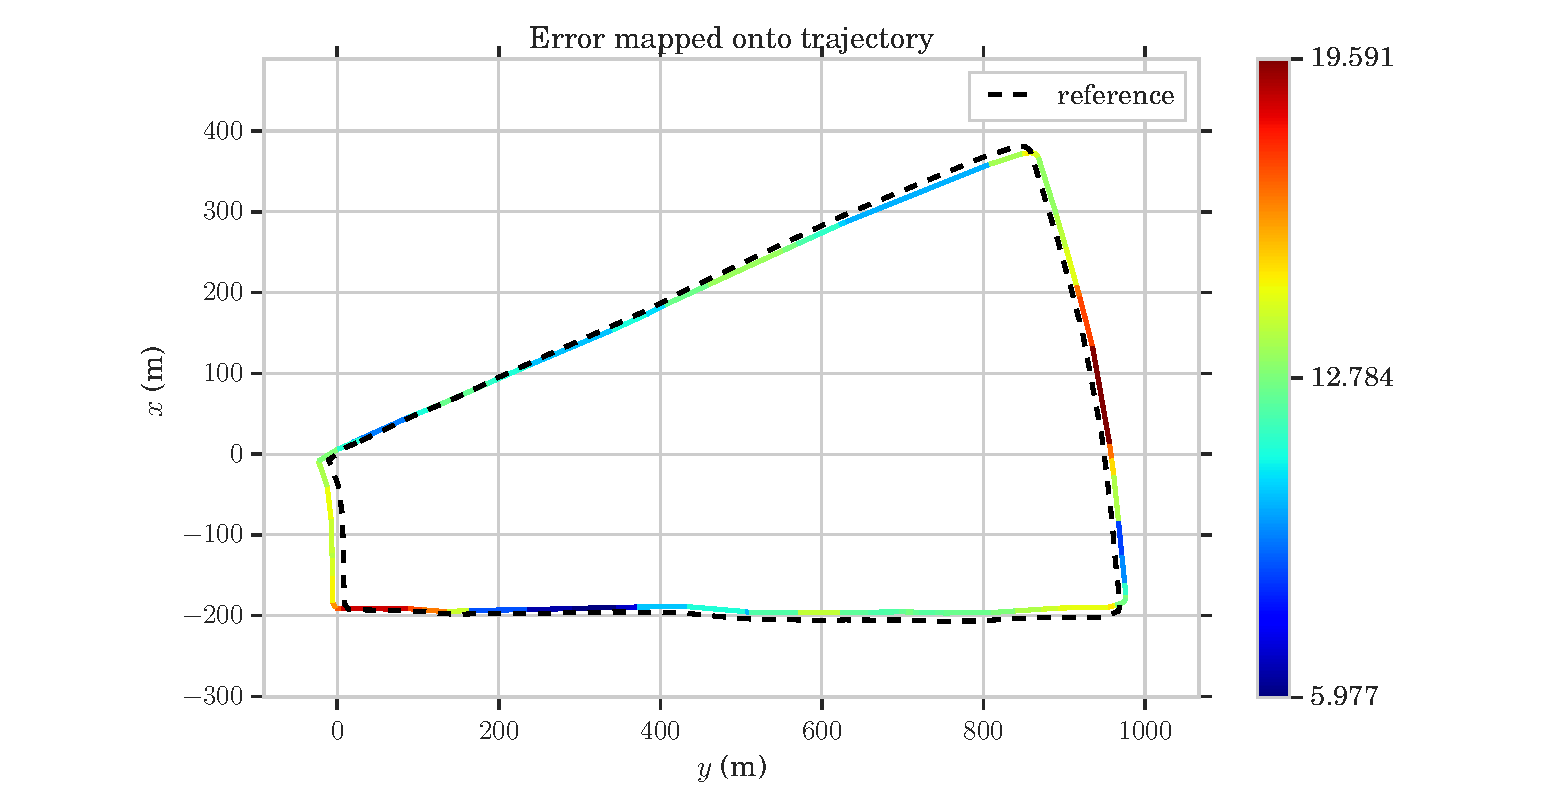
\includegraphics[width=0.90\textwidth]{figures/chapter5/ape_map_3km}
	\caption{本地实验一的二维定位绝对误差图}\label{fig5_17}
\end{figure}\newpage
\begin{figure}[!h]\setlength{\belowcaptionskip}{-12pt}
	\centering
	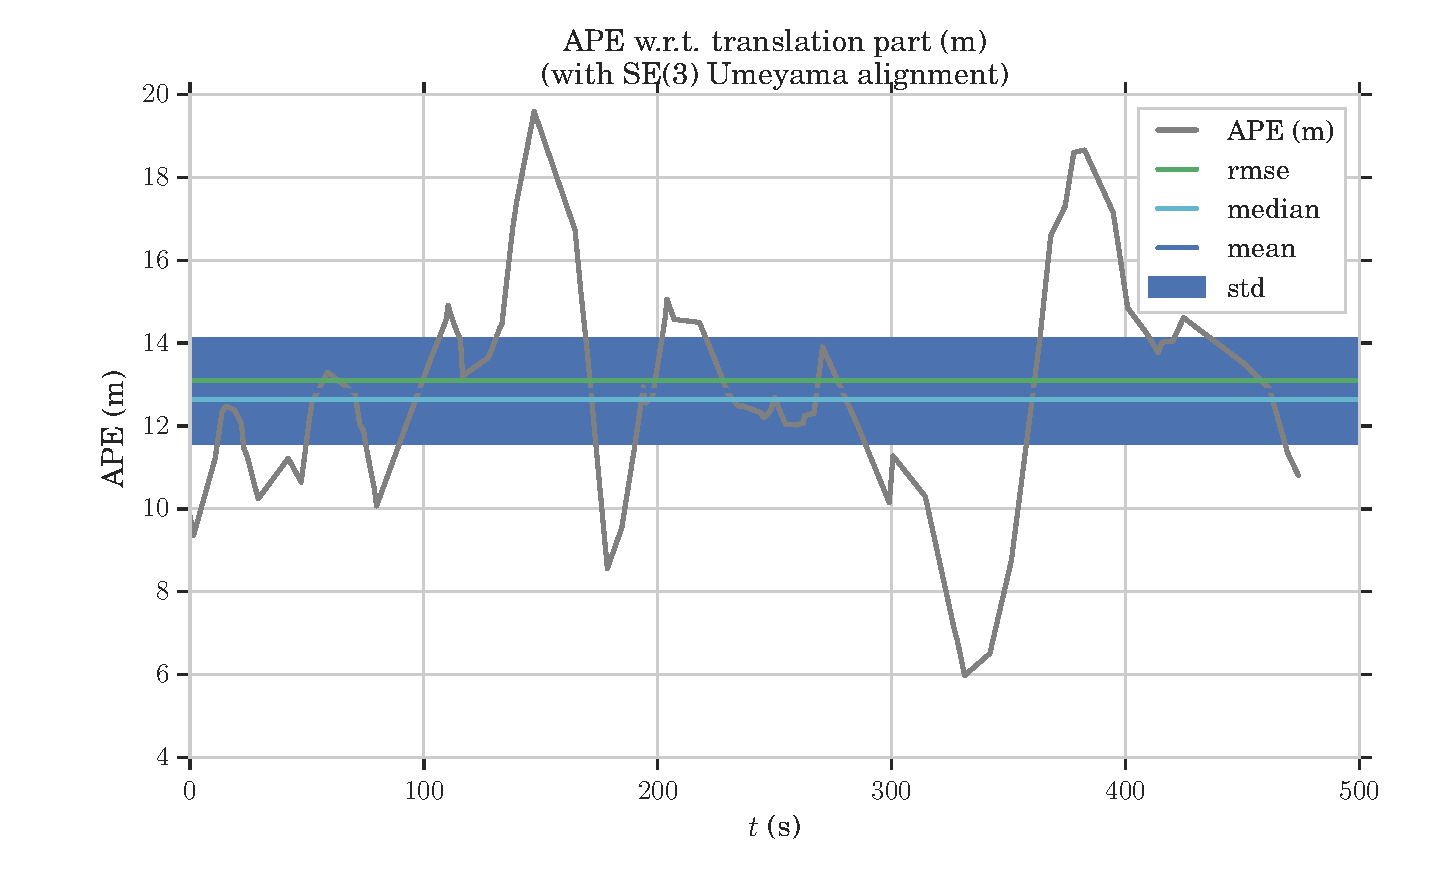
\includegraphics[width=1.0\textwidth]{figures/chapter5/ape_err_3km}
	\caption{本地实验一的系统定位误差指标图}\label{fig5_18}
\end{figure}
\begin{table}[!h]\setlength{\abovecaptionskip}{6pt}
	\zihao{5}
	\centering
	\caption{本地实验一的系统定位误差指标} \label{tab:5.3}
	\begin{tabular*}{0.9\textwidth}{@{\extracolsep{\fill}}cccccc}
		\toprule
		APE\_MAX(m)&APE\_MIN(m) &RMSE	&STD	&MEAN(m)	&MEDIAN(m) \\
		\midrule
		19.5912	 &5.9771	&13.0965	&2.5359	 &12.8487	&12.6319 \\
		\bottomrule
	\end{tabular*}
\end{table}

可见,本地实验一的最大定位误差是19.5912米,定位精度≤0.6\%。\newpage
\subsection{本地实验二}
实验二的行车轨迹如图\ref{fig5_14}红线所示。图\ref{fig5_19}是二维定位轨迹图对比图,图\ref{fig5_20}是二轴位置(x, y)对比图。其中VI\_SLAM是本系统输出轨迹,RTK是差分GPS轨迹。通过图\ref{fig5_19}和图\ref{fig5_20},可以定性分析系统的定位误差。
\begin{figure}[h]\setlength{\belowcaptionskip}{-12pt}
	\centering
	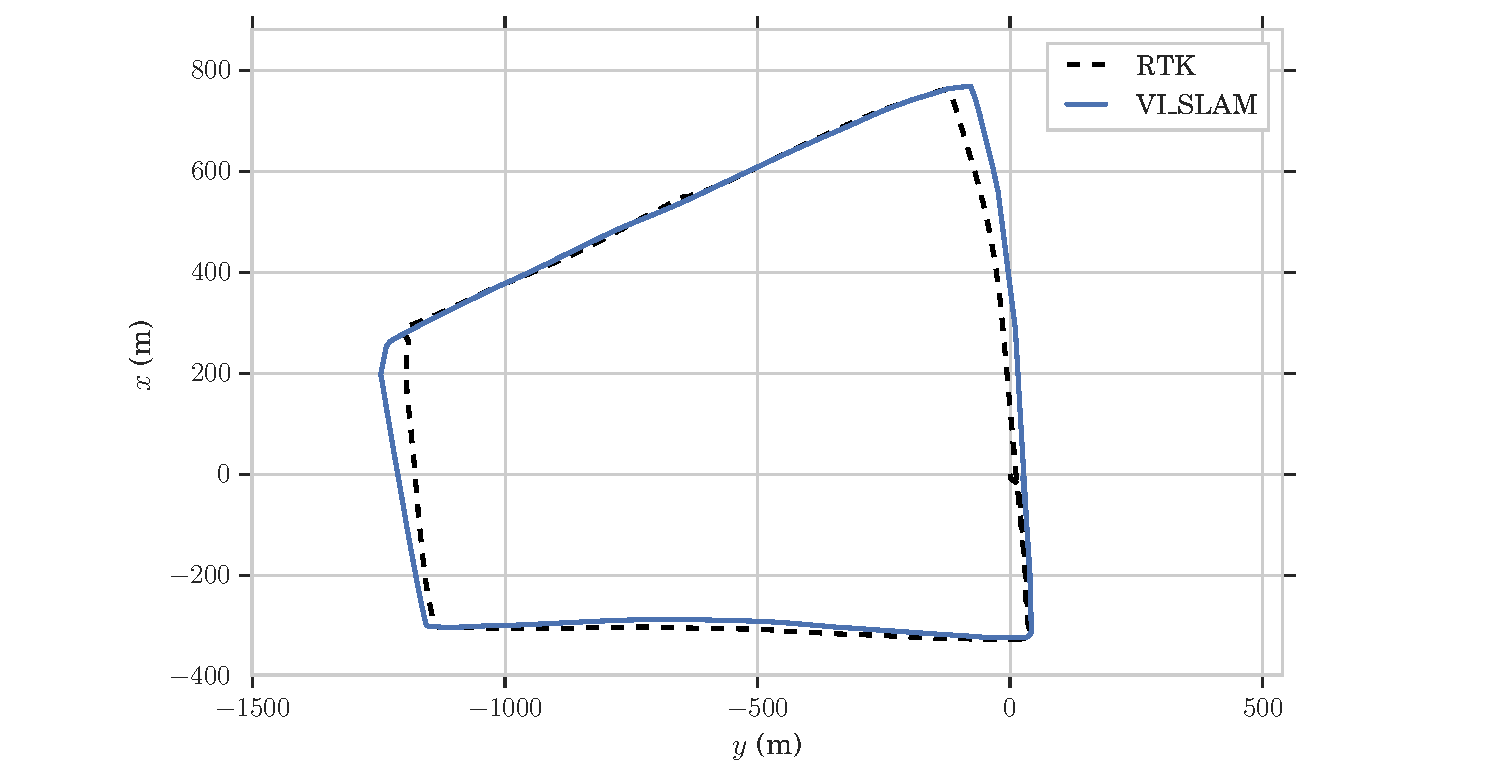
\includegraphics[width=0.90\textwidth]{figures/chapter5/traject_5km}
	\caption{本地实验二的二维定位轨迹图对比图}\label{fig5_19}
\end{figure}
\begin{figure}[h]\setlength{\belowcaptionskip}{-12pt}
	\centering
	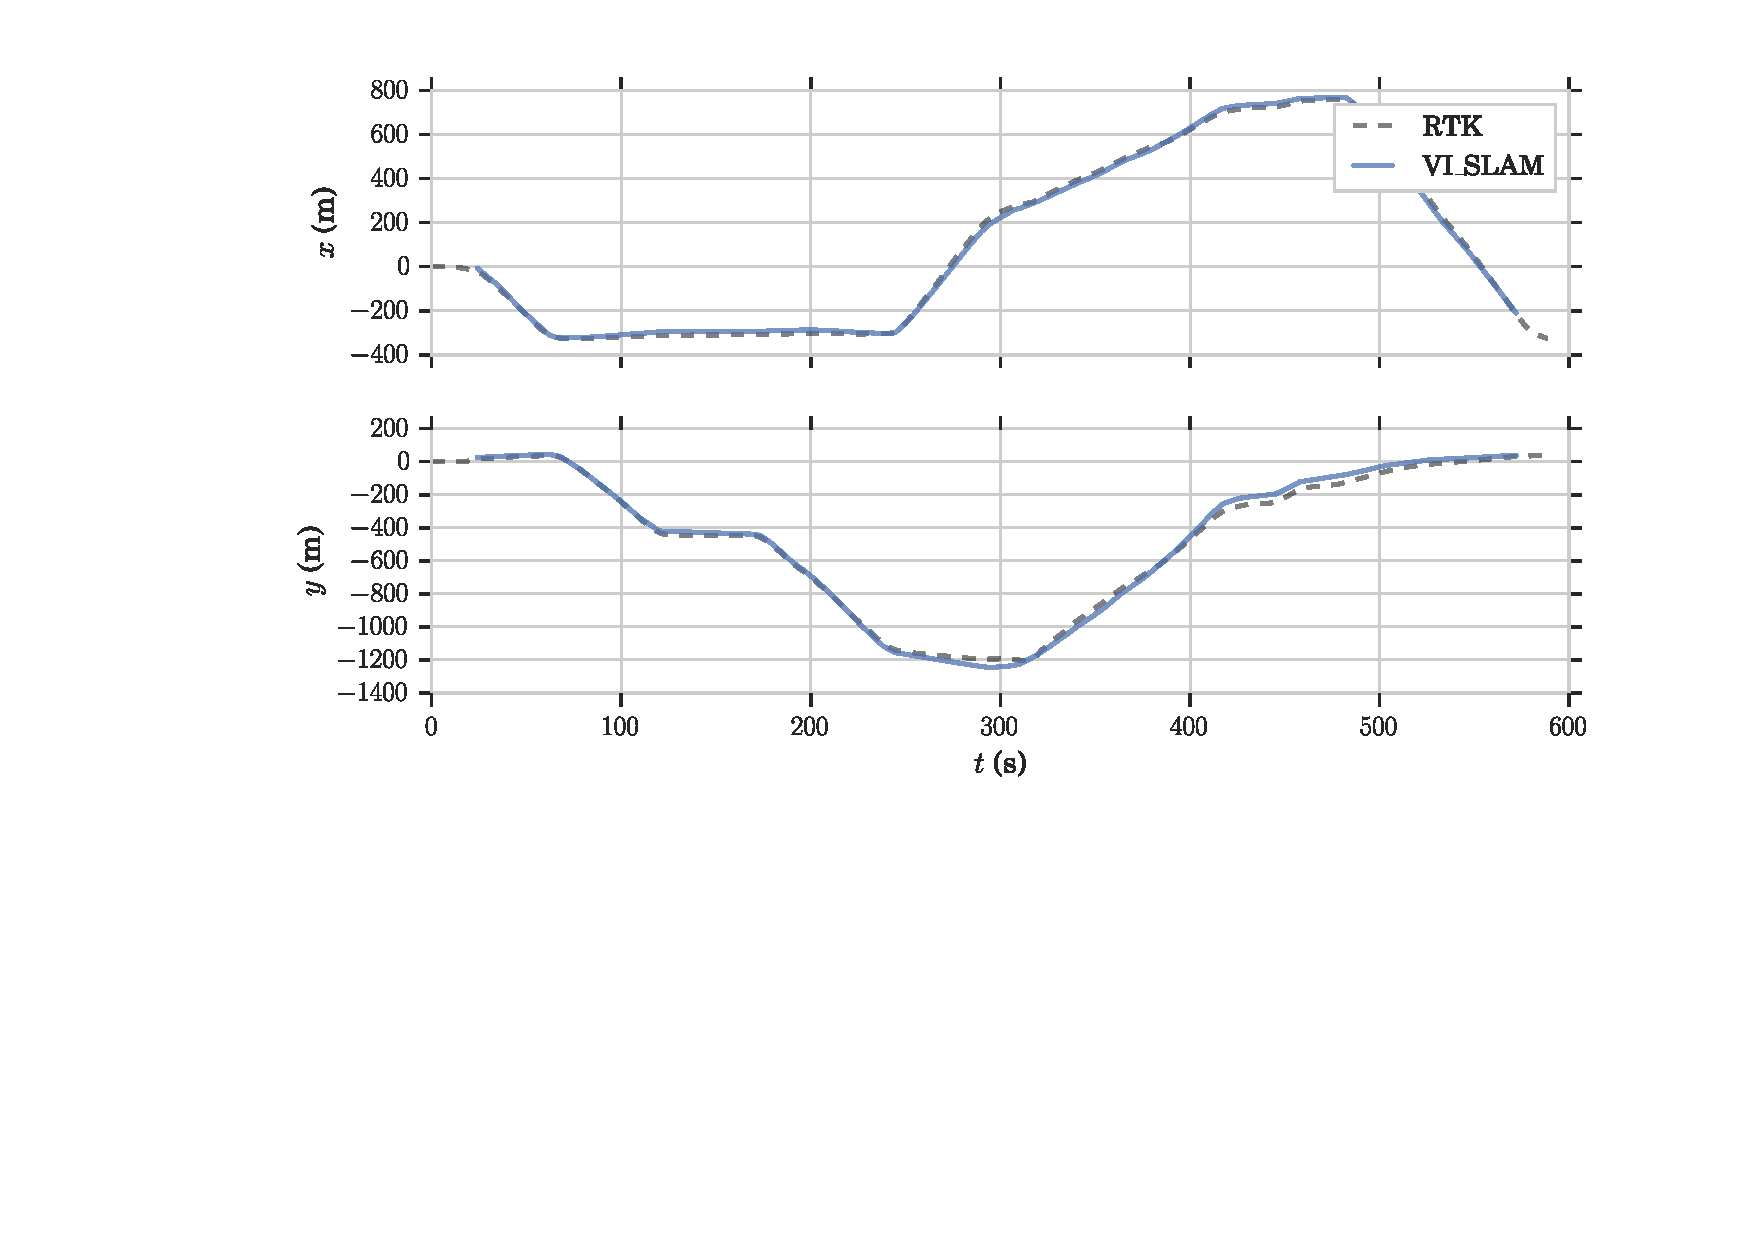
\includegraphics[width=1.0\textwidth]{figures/chapter5/xy_5km}
	\caption{本地实验二的二维位置(x, y)对比图}\label{fig5_20}
\end{figure}

然后定量分析本地实验二中系统的定位误差。图\ref{fig5_21}是二维定位绝对误差图。同样,计算出APE,RMSE,STD,MEAN和MEDIAN,将计算结果展示在表\ref{tab:5.4}中。为了更加直观,将这些误差以曲线图的形式展示出来,如图\ref{fig5_22}所示。\newpage
\begin{figure}[!h]
	\centering
	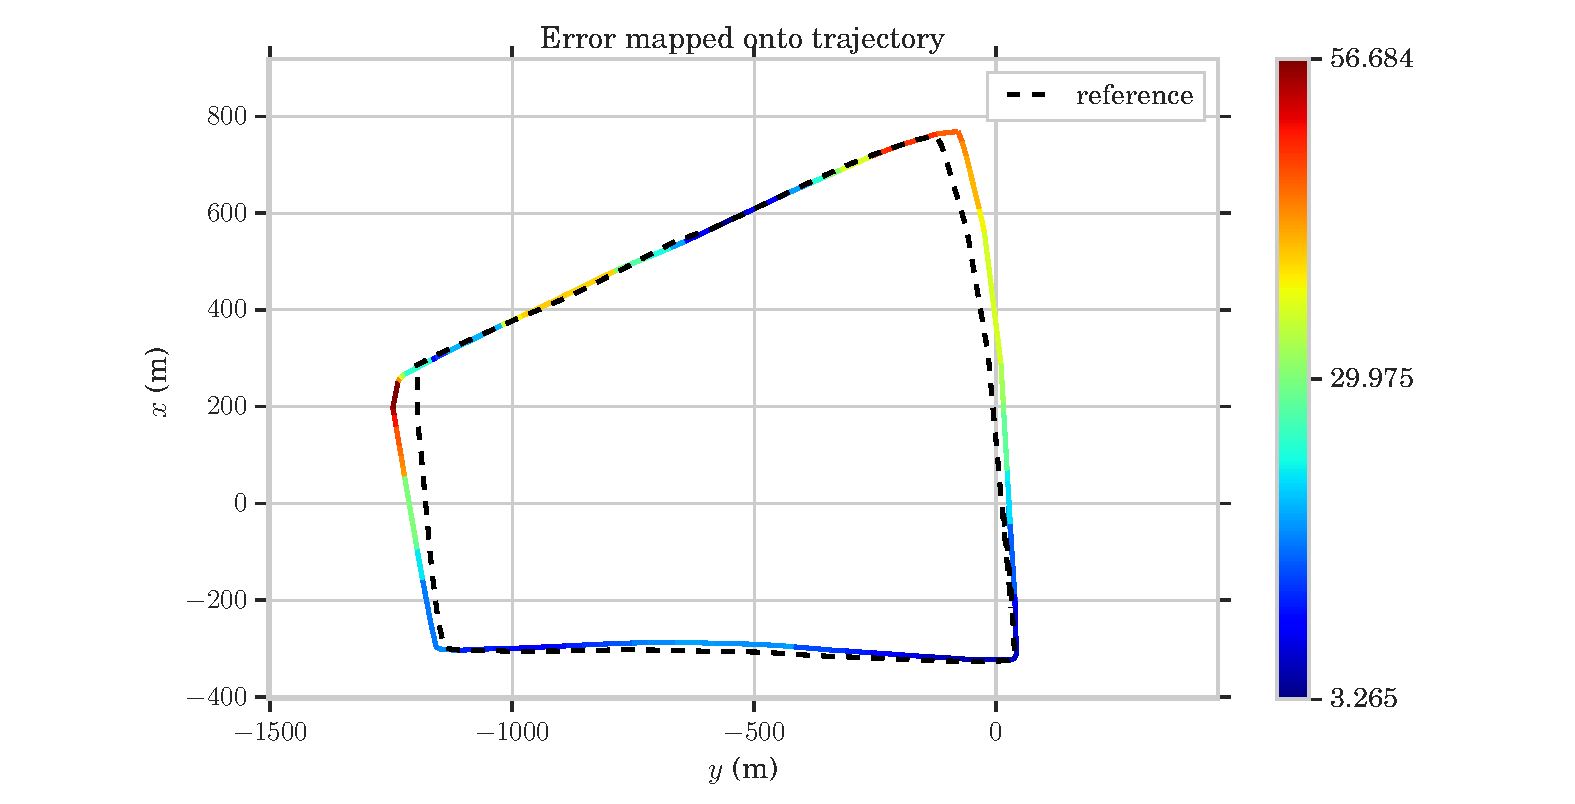
\includegraphics[width=0.90\textwidth]{figures/chapter5/ape_map_5km}
	\caption{本地实验二的二维定位绝对误差图}\label{fig5_21}
\end{figure}
\begin{figure}[!h]\setlength{\belowcaptionskip}{-12pt}
	\centering
	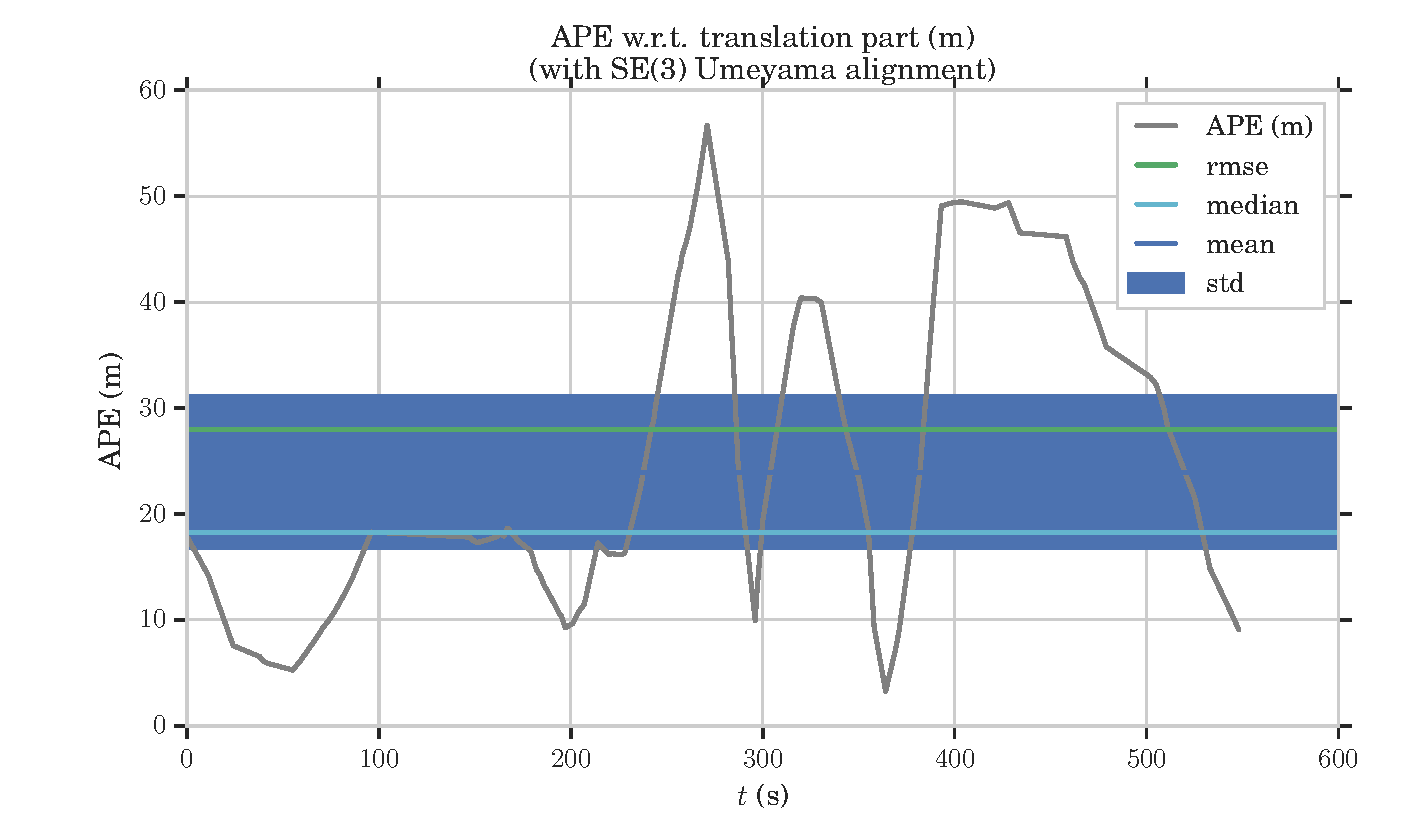
\includegraphics[width=0.85\textwidth]{figures/chapter5/ape_err_5km}
	\caption{本地实验二的系统定位误差指标图}\label{fig5_22}
\end{figure}
\begin{table}[!h]\setlength{\abovecaptionskip}{6pt}
	\zihao{5}
	\centering
	\caption{本地实验二的系统定位误差指标} \label{tab:5.4}
	\begin{tabular*}{0.9\textwidth}{@{\extracolsep{\fill}}cccccc}
		\toprule
		APE\_MAX(m)&APE\_MIN(m) &RMSE	&STD	&MEAN(m)	&MEDIAN(m) \\
		\midrule
		56.6838	&3.2654	&27.9445	&14.3974	&23.9501	&18.2750 \\
		\bottomrule
	\end{tabular*}
\end{table}

可见,本地实验二的最大定位误差是56.6838米,定位精度≤1.3\%。相比于本地实验一,定位精度有所下降。
\section{本章小结}
本章通过实验验证了本系统的定位效果。首先使用EuRoc数据集,验证了本系统在三维空间中的定位效果。然后进行本地校园车载实验,验证了本系统在大地平面上的定位效果。其中,EuRoc是室内环境,飞行距离短,环境简单。校园车载实验是室外环境,行驶路线长,环境复杂多变。两种环境下的实验数据说明本系统在不同的环境下都能正常工作,在短距离情况下定位精度较高,但是随着距离的增加,绝对定位精度会逐渐下降。